%!TEX root = main.tex
\clearpage
\begin{refsection}
%\renewcommand*{\thepage}{A\arabic{page}}
\beginsupplement
\appendix
\pagenumbering{arabic}
\begin{center}
\textbf{\large Supplemental Materials: On the use of rank percentile in evaluating scientific impacts, and its predictability}

Panos Ipeirotis, Sen Tian
\end{center}

\section{The robustness of rp.rp5}
\label{sec:robustness_rprp}
The evaluation metric to formulate rp.rp5$_{i\tau}$ is an aggregation of the performances of all the publications that the author publish by age $\tau$. And to be more specific, we use rp.c$_{j5}$ to evaluate publication $j$, and the evaluation metric is given as the sum of all papers published by $\tau$, i.e. m.rp5$_{i\tau} = \sum_{j=1}^{N_\tau^{(i)}} \text{rp.c}_{j5}$ (the notation m.rp5 is to distinguish from other metrics we are going to study below). rp.c$_{j5}$ only utilizes the citation history of a publication in the first $5$ years. This may not seems to be adequate to represent the quality of a paper. However, as we show in figure \ref{fig:scatter_pubrp_bio1980}, rp,c is highly stable over ages, i.e. rp.c$_{j5}$ is likely to be close to rp.c$_{j10}$ for majority of the papers. 

We can consider other ways of summarizing the performance of a paper, and we show that not only such metrics have high correlations with m.rp5, but the rank percentile indicators based on these metrics are not statistically significantly different from rp.rp5. Consider the entire history that we have for publication $j$: rp.c$_{j1}$, rp.c$_{j2}$, $\cdots$, rp.c$_{j T_j}$. Besides evaluating the publication at certain age, we can use the summary statistic to take advantage of the entire history. For example, we can take the best performance throughout its career, i.e. $\displaystyle \max_{t=1,\cdots,T_j} \text{rp.c}_{jt}$, and aggregate them to formulate the evaluation metric, i.e. m.rpmax$_{i\tau} = \displaystyle \sum_{j=1}^{N_\tau^{(i)}} \max_{t=1,\cdots,T_j} \text{rp.c}_{jt}$. The correlation between m.rp5 and m.rpmax at each fixed age $\tau=1,\cdots,30$ is displayed in figure \ref{fig:robustness_test_cor}, and we can see that these two metrics are highly correlated. Meanwhile, other choices of the evaluation metrics also have high correlations with m.rp5 according to the figure. Furthermore, we construct rp.rpmax based on m.rpmax and study its difference with rp.rp5. We perform a paired t-test on the two samples rp.rpmax and rp.rp5 at each fixed age $\tau=1,\cdots,30$. The p-values that we get are all extremely close to $1$, which indicates that the difference between rp.rpmax and rp.rp5 is not significant. Similar results are obtained for other types: rp.rpmean, rp.rpmedian and rp.rp10. 


\iffalse
\begin{equation}
\label{eq:rp_matrix}
\bordermatrix{
    & \text{age 1}     & \text{age 2}     & \cdots & \text{age $K$}     \cr
    \text{paper 1}     & \text{rp}_{11}^{(c)}     & \text{rp}_{12}^{(c)}     & \ldots & \text{rp}_{1 K}^{(c)}      \cr
    \text{paper 2}     & \text{rp}_{21}^{(c)}     & \text{rp}_{22}^{(c)}    & \ldots & \text{rp}_{2 K}^{(c)}     \cr
    \quad \vdots & \vdots & \vdots & \ddots & \vdots \cr
    \text{paper $N$}     & \text{rp}_{N 1}^{(c)}     & \text{rp}_{N 2}^{(c)}     & \ldots  & \text{rp}_{N K}^{(c)}    \cr
}
\end{equation}

We take the maximum performance for each of the $N$ papers, and sum them:
\begin{equation}
    \omega_{i \tau} = \sum_{j=1,\cdots,N} \max_{k=1,\cdots, K} \text{rp}_{j k} ^{(c)}.
\end{equation}
\fi

\section{Stationarity test}
\label{sec:stationarity_test}
Two commonly used statistical tests for stationarity are the Dicky-Fuller test\supercite{dickey1979distribution} and KPSS test\supercite{kwiatkowski1992testing}. Two tests formulate the hypothesis testing problem differently. Dicky-Fuller test assumes a unit root is present in the series. A unit root means the series is $I(1)$, i.e. integrated order $1$ and the first differenced series is stationary. The more negative the test statistic is, the stronger the rejection of the null. On the other hand, KPSS test assumes the null as the series being stationary, i.e. $I(0)$. KPSS test is slightly more general since it allows testing a series being non-stationary but doesn't present a unit root. The more positive the test statistic is, the stronger the rejection of the null. Both tests include the drift in the test equations but exclude the trend, since we do not observe significant trends in the series. 

We apply these tests on each individual rp series. The test statistics are shown in figure \ref{fig:stationarity_test}. The dashed lines indicate the critical values at $5 \%$ level. KPSS test indicates that rp$^{(c)}$ and rp.rp5$^{(c)}$ are non-stationary, and we don't have enough evidence to reject them being $I(1)$ according to the Dicky-Fuller test. Meanwhile, the differenced series are stationary based on both tests.

\printbibliography[heading=subbibliography]


\clearpage
\section{Tables and figures}
\begin{table}[htbp]
  \centering
    \begin{tabular}{l|l}
    Method & Tuning parameters \\
    \midrule
    LASSO & Penalty strength parameter \\
    \midrule
    Ridge & Penalty strength parameter \\
    \midrule
    \multirow{2}[2]{*}{Elastic net} & Penalty strength parameter \\
          & Penalty gap parameter \\
    \midrule
    \multirow{2}[2]{*}{Gamma LASSO} & Penalty strength parameter \\
          & Convexity parameter \\
    \midrule
    \multirow{3}[2]{*}{Random forest} & Number of trees to grow \\
          & Number of variables used at each split \\
          & Minimum number of observations in a node \\
    \midrule
    \multirow{9}[2]{*}{xgbtree} & Maximum number of iterations \\
          & Learning rate \\
          & Regularization parameter \\
          & Maximum depth of the tree \\
          & Minimum number of observations in each child leaf \\
          & Number of observations supplied to a tree \\
          & Number of features supplied to a tree \\
          & Regularization parameter for ridge penalty \\
          & Regularization parameter for LASSO penalty \\
    \midrule
    \multirow{5}[1]{*}{Deep neural network} & Number of layers  \\
          & Learning rate \\
          & Number of hidden units at each layer \\
          & Dropout rate \\
          & Regularization parameter \\
    \end{tabular}%
  \caption{Hyper-parameter(s) of the machine learning models.}
  \label{tab:hyperpara}%
\end{table}%

\begin{table}[htbp]
  \centering
    \begin{tabular}{l|l}
    Feature & Description \\
    \midrule
    pub\_cit\_cumulative & total citations of publication $j$ \\
    pub\_cit\_yearly & citations of publication $j$ at age $\tau_1$ \\
    pub\_cit\_peryear & average citations of publication $j$ per age \\
    pub\_rp\_cumulative & rank percentile indicator calculated based on total citations, i.e. rp.c$_{j\tau_1}$ \\
    pub\_rp\_yearly & rank percentile indicator calculated based on yearly citations \\
          &  \\
    aut\_cit\_cumulative          & total citations of author $i$ \\
    aut\_cit\_yearly          & citations of author $i$ at age $\tau_1$ \\
    aut\_npub\_cumulative & total number of publications of author $i$ \\
    aut\_npub\_yearly & number of publications of author $i$ at age $\tau_1$ \\
    aut\_cit\_perpaper & average citations per paper of author $i$  \\
    aut\_h\_index & h-index of author $i$  \\
    aut\_g\_index & g-index of author $i$ \\
    aut\_maxcit\_pub & largest citations that a single paper of author $i$ has received \\
    aut\_rprp5\_cumulative & author rank percentile calculated based on all papers, i.e. rp.rp5$_{i\tau_1}$ \\
    aut\_rprp5\_yearly & author rank percentile calculated based on papers written at $\tau_1$ \\
          &  \\
    *\_delta & the difference over the last two ages for each of the above features \\
    \end{tabular}%
  \caption{Features for predicting the impact of publication $j$. The features are created at $\tau_1$.}
  \label{tab:features_pubrp}%
\end{table}%

\begin{table}[htbp]
  \centering
    \begin{tabular}{l|l}
    Feature & Description \\
    \midrule
    aut\_cit\_cumulative & total citations of author $i$ \\
    aut\_cit\_yearly & citations of author $i$ at age $\tau_1$ \\
    aut\_npub\_cumulative & number of publications of author $i$ \\
    aut\_npub\_yearly & number of publications of author $i$ at age $\tau_1$ \\
    aut\_h\_index & h-index of author $i$ \\
    aut\_g\_index & g-index of author $i$ \\
    aut\_cit\_peryear & average citations per age of author $i$ \\
    aut\_rprp5\_cumulative & author rank percentile calculated using all publications, i.e. rprp5$_{i\tau_1}$ \\
    aut\_rprp5\_yearly & author rank percentile calculated using publications written in age $\tau_1$ \\
          &  \\
    pub\_cit\_cumulative\_\{min,mean,max\} & citations received by each of the publications \\
    pub\_cit\_yearly\_\{min,mean,max\} & citations received by each of the publications written in age $\tau_1$ \\
    pub\_rp\_cumulative\_\{min,mean,max\} & publication rank percentiles calculated based on total citations \\
    pub\_rp\_yearly\_\{min,mean,max\} & publication rank percentiles calculated based on citations in age $\tau_1$ \\
          &  \\
    *\_delta & the difference over the last two ages for each of the above features \\
    \end{tabular}%
  \caption{Features for predicting the impact of author $i$. The features are created at $\tau_1$.}
  \label{tab:features_autrp}%
\end{table}%

% exploratory plots of the data
\begin{figure}[ht!]
    \centering
    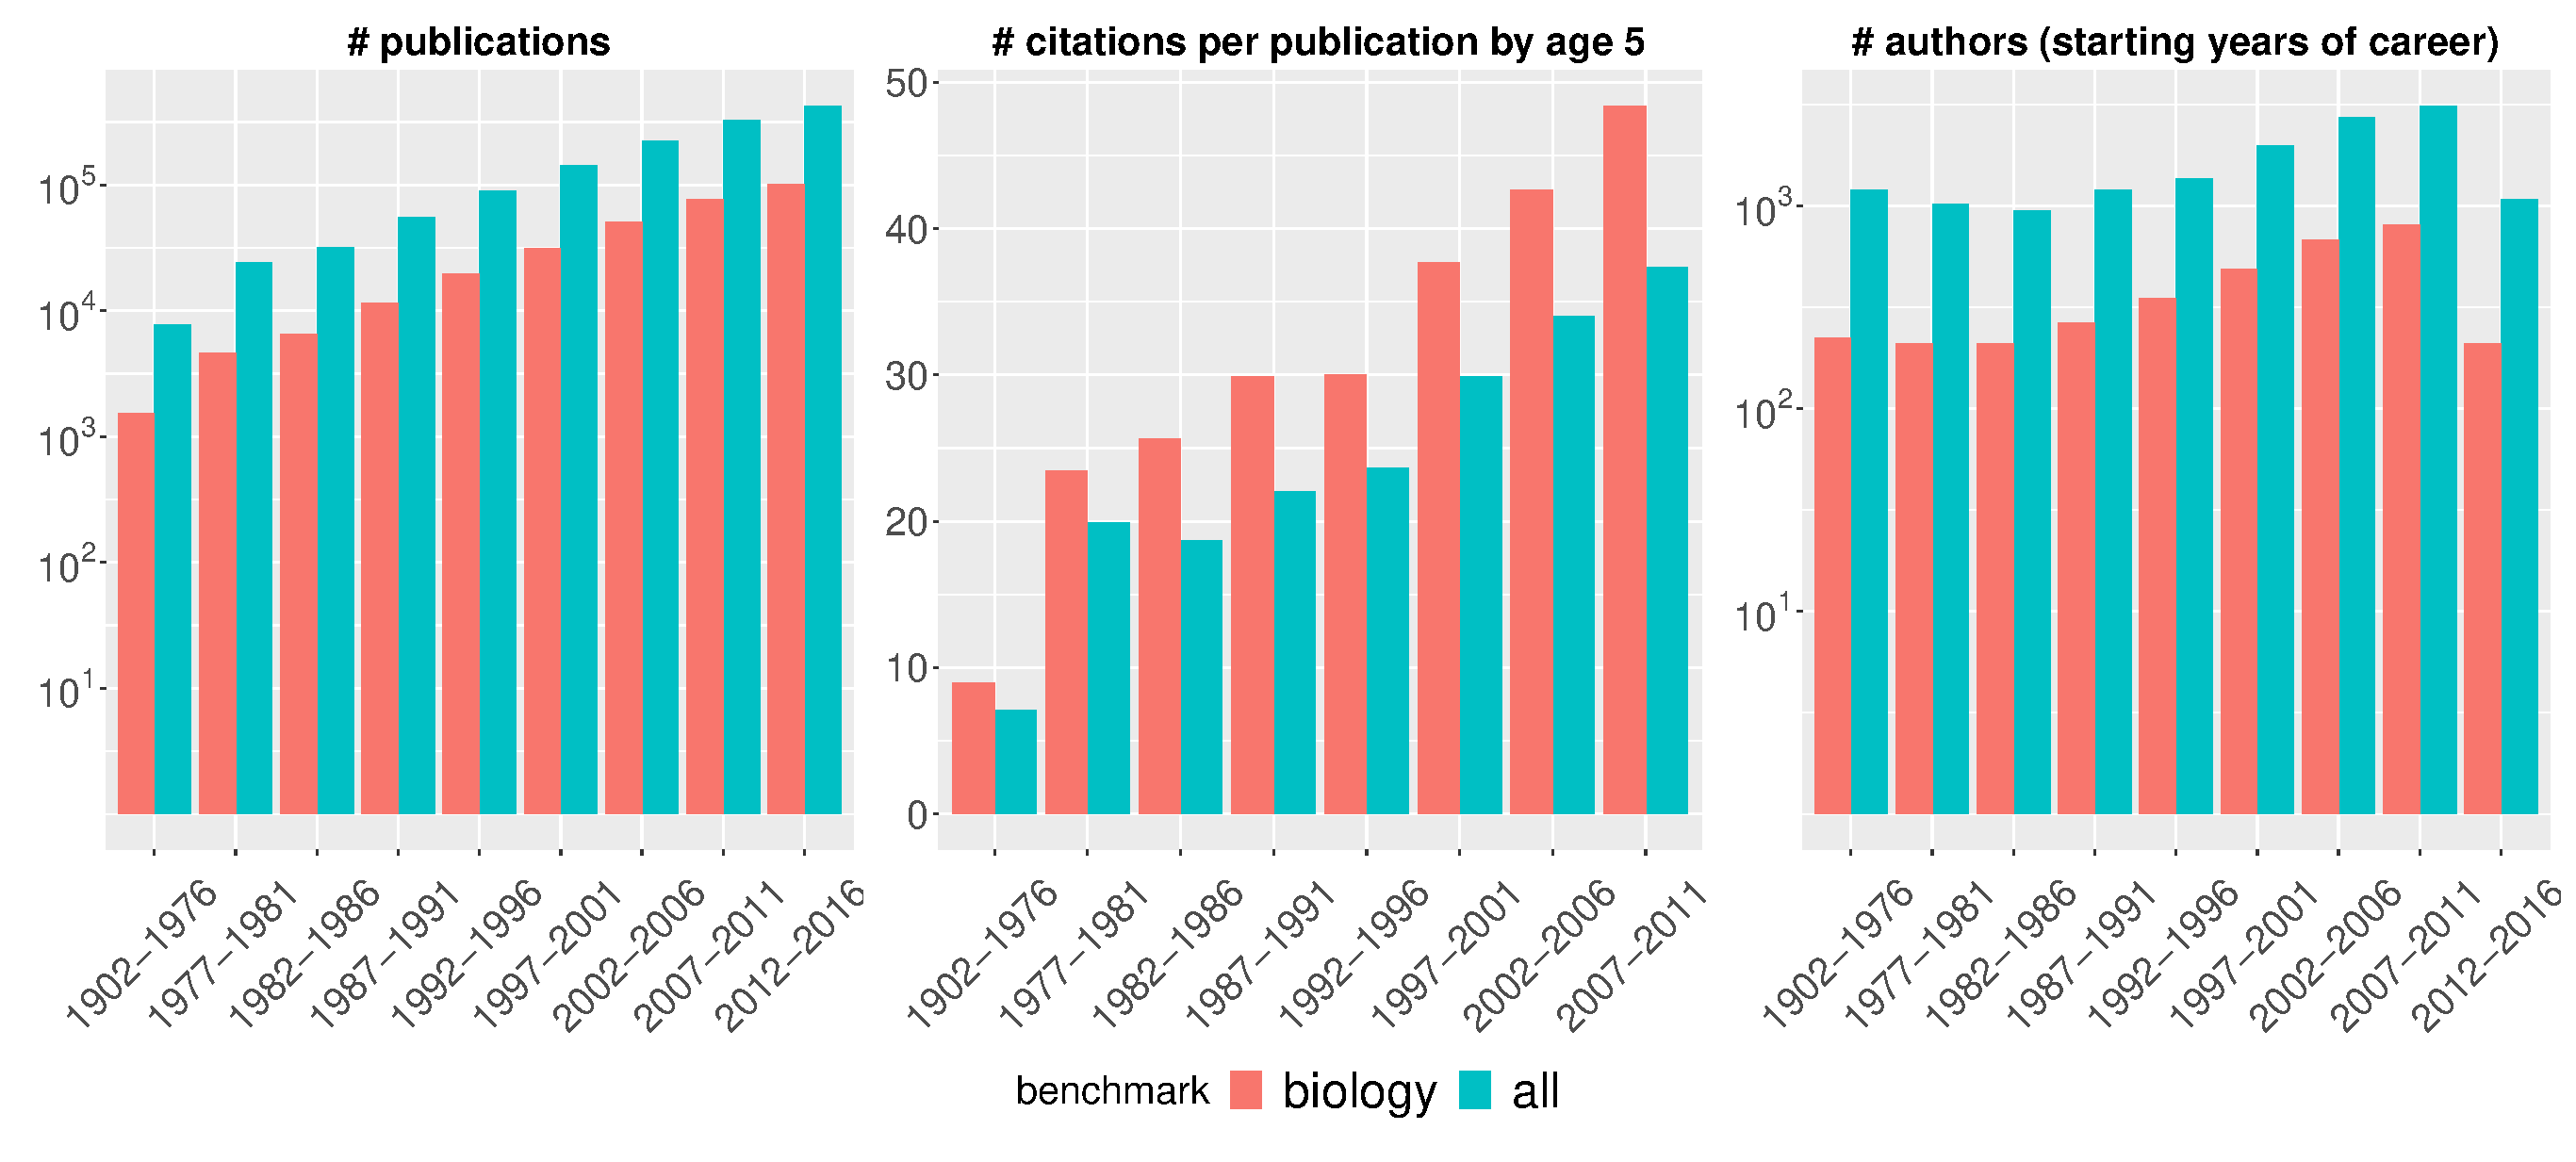
\includegraphics[width=\textwidth]{figures/exploratory/npub_ncitperpub_naut.eps}
    \caption{\textbf{Left panel}: number of publications; \textbf{middle panel}: average number of citations per publication by age $5$, for papers published in a certain period; \textbf{right panel}: number of authors who start their careers in a certain period. Newer publications have more citations (on average) than the older ones, due to the seniority effect of an author. The authors in our dataset remain active by year $2016$ and their publications in the early stage of career is usually less recognizable and attracts less citations, than those published more recently. Meanwhile, publications in biology generally have more citations per paper, which corresponds to the fact that biology is a highly productive field and it attracts a large number of citations.}
    \label{fig:exploratory}
\end{figure}

% publication rank percentile, heat map of correlations
\begin{figure}[ht!]
    \centering
    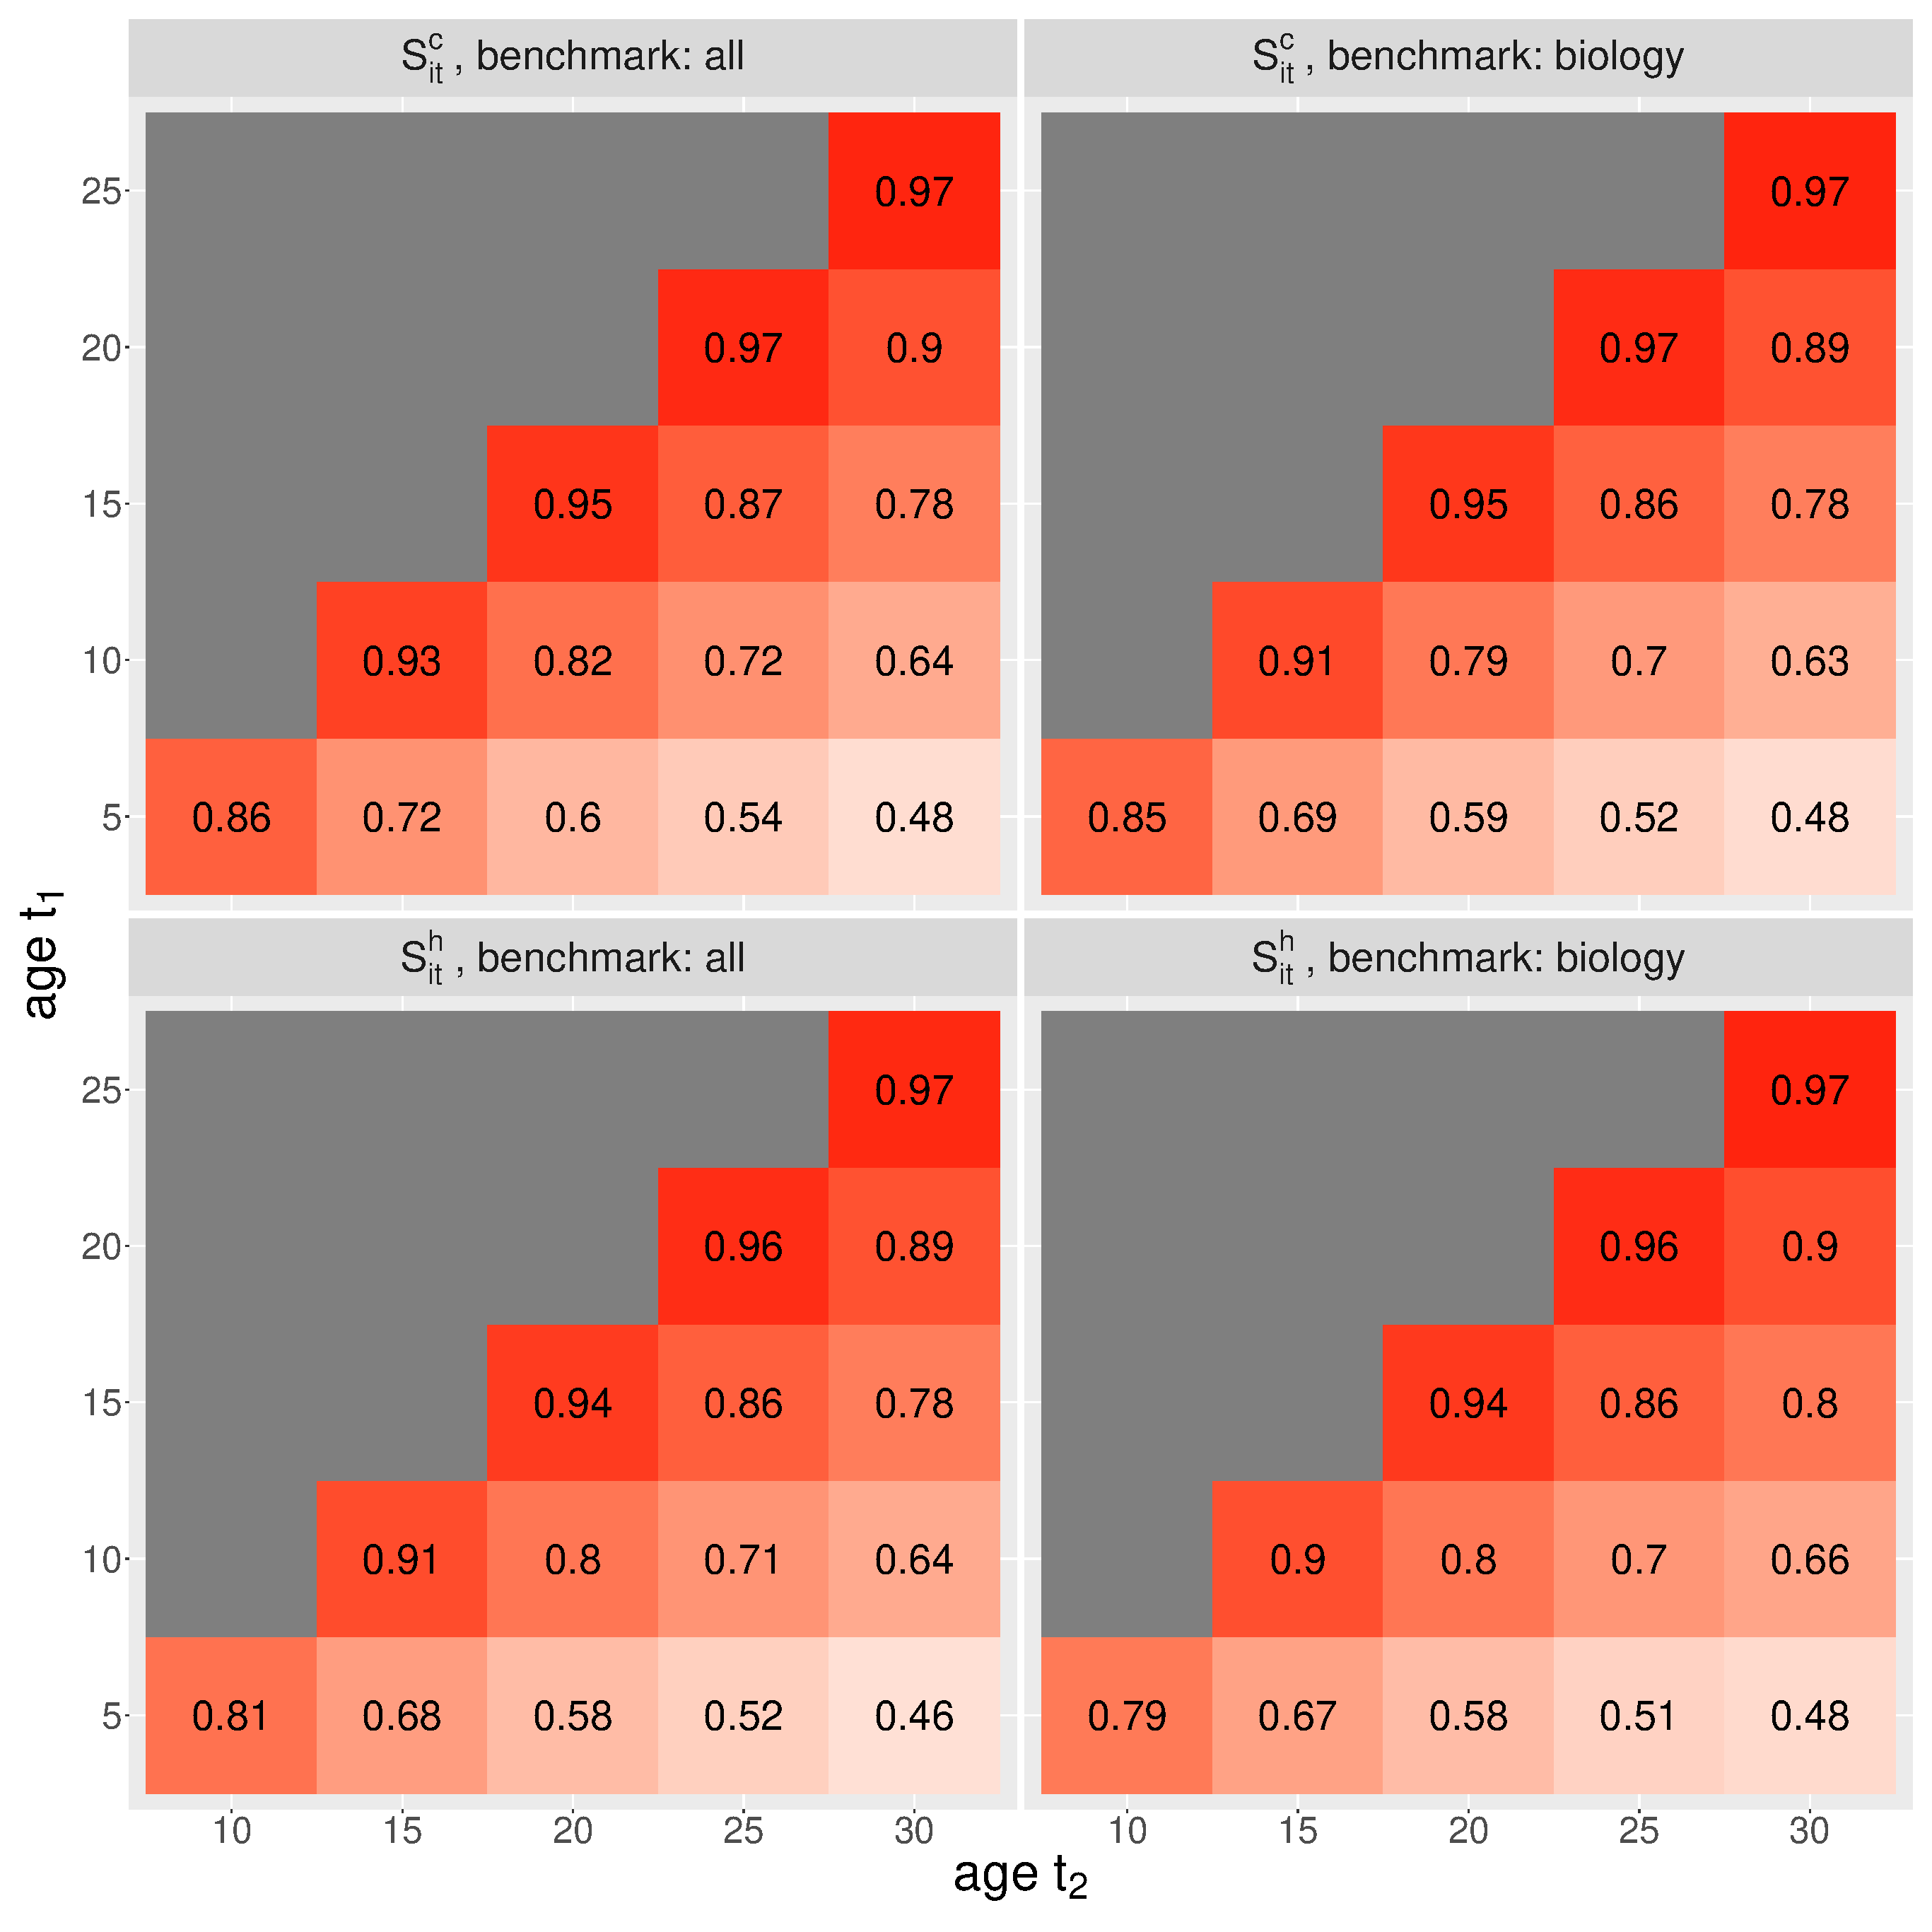
\includegraphics[width=\textwidth]{figures/pred_power/current/heatmap_cor_autrp.eps}
    \caption{The Pearson's correlation between rp indicators at two different ages. The benchmark either includes all publications or only publications in biology.}
    \label{fig:hm_autrp_current}
\end{figure}


\begin{figure}[ht!]
    \centering
    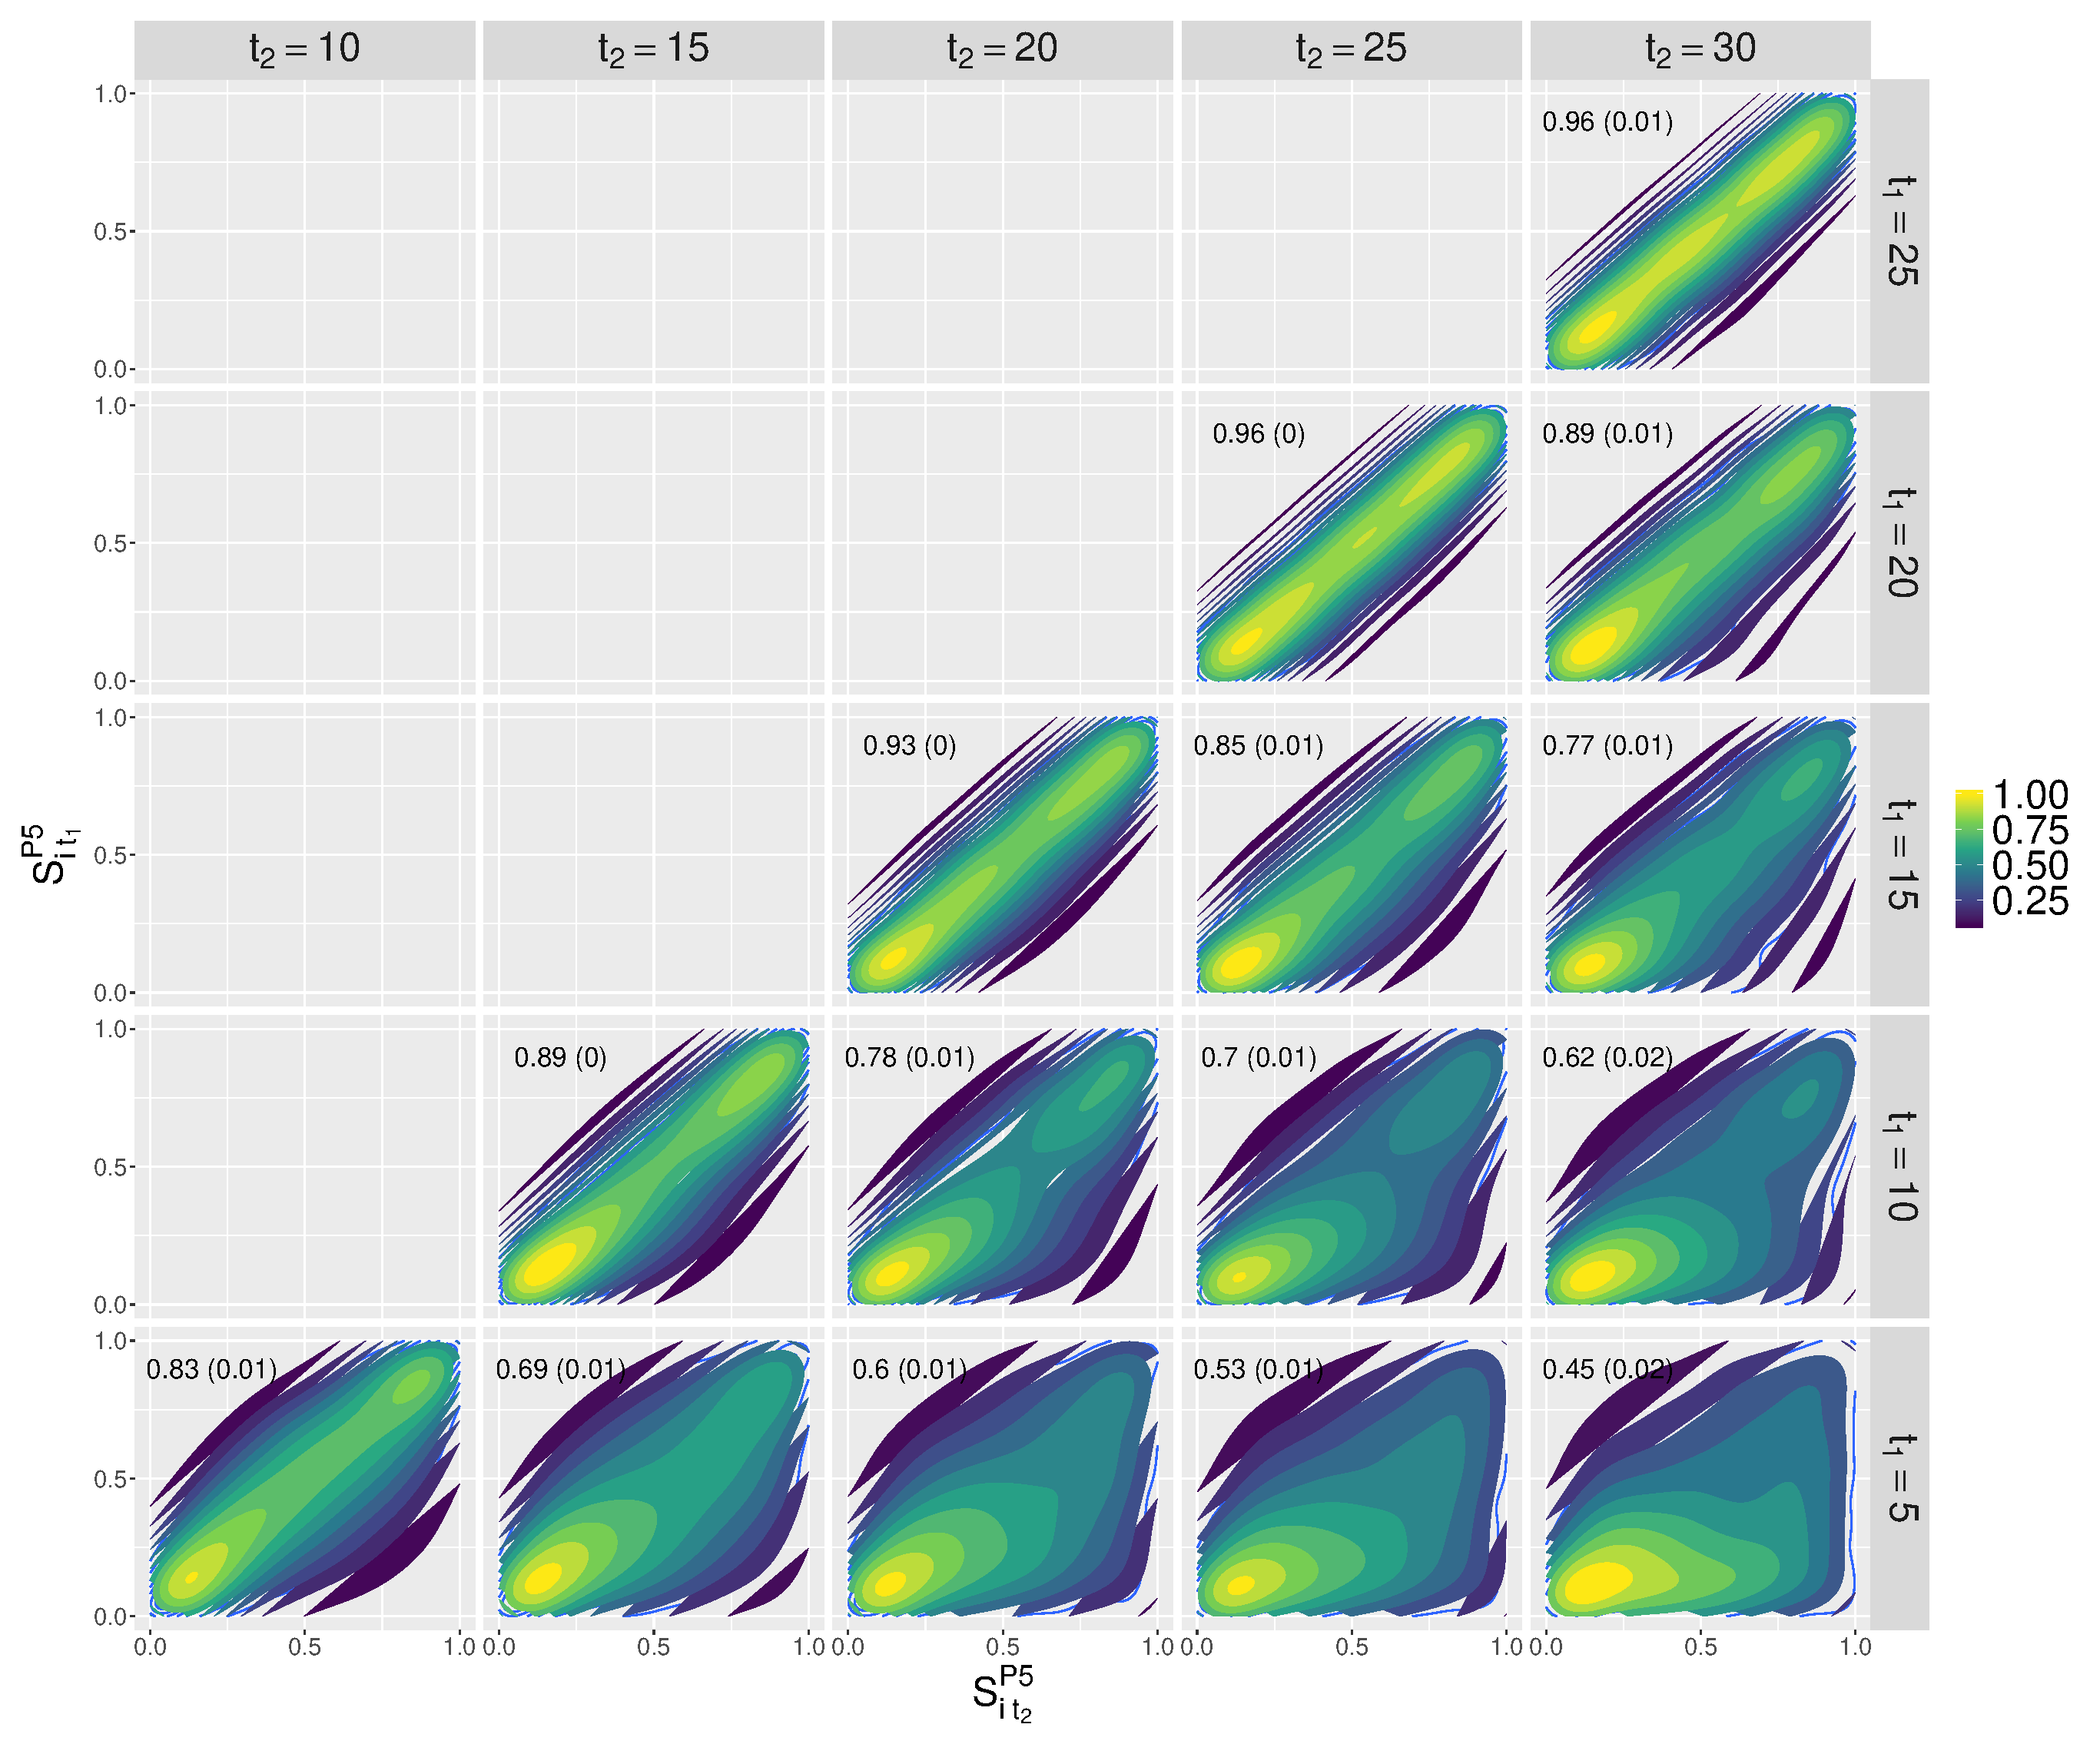
\includegraphics[width=\textwidth]{figures/pred_power/autrp/scatter_all.eps}
    \caption{Kernel density estimation of the scatters of S$_{i t_1}$ and S$_{i t_2}$. Meanwhile, we fit a simple linear regression of S$_{i t_2}$ upon S$_{i t_1}$. The estimated coefficient and the corresponding standard error (in the bracket) are displayed in each facet. The benchmark here is all.}
    \label{fig:scatter_autrp_all}
\end{figure}

\begin{figure}[ht!]
    \centering
    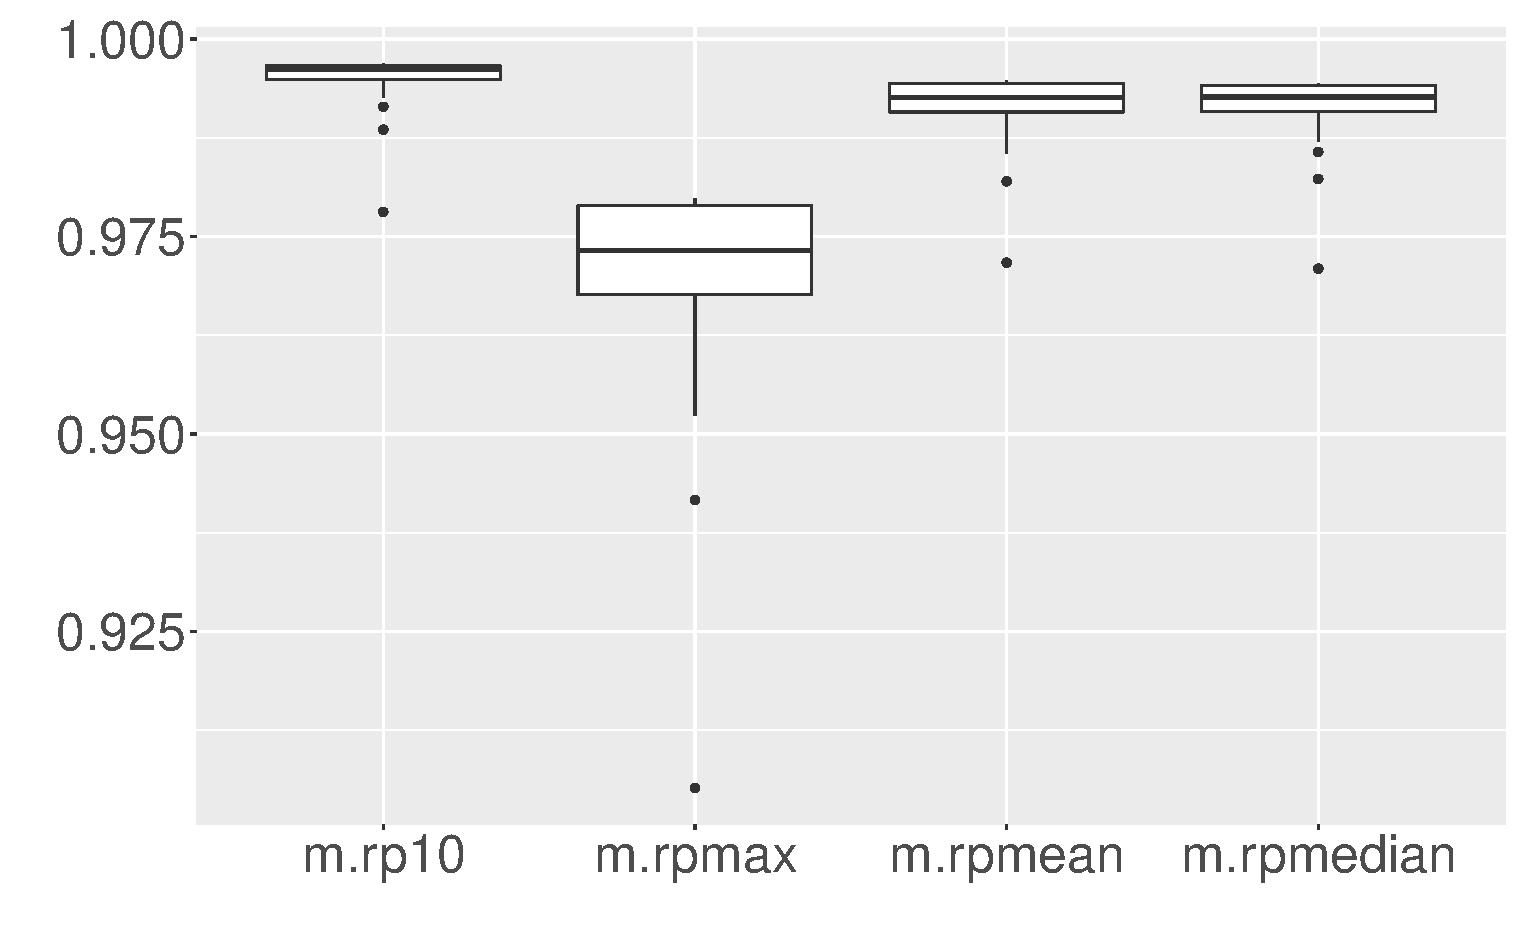
\includegraphics[width=0.7\textwidth]{figures/robustness_test/cor.eps}
    \caption{Pearson's correlation between m.rp5 and other evaluation metrics.}
    \label{fig:robustness_test_cor}
\end{figure}


\begin{figure}[ht!]
    \centering
    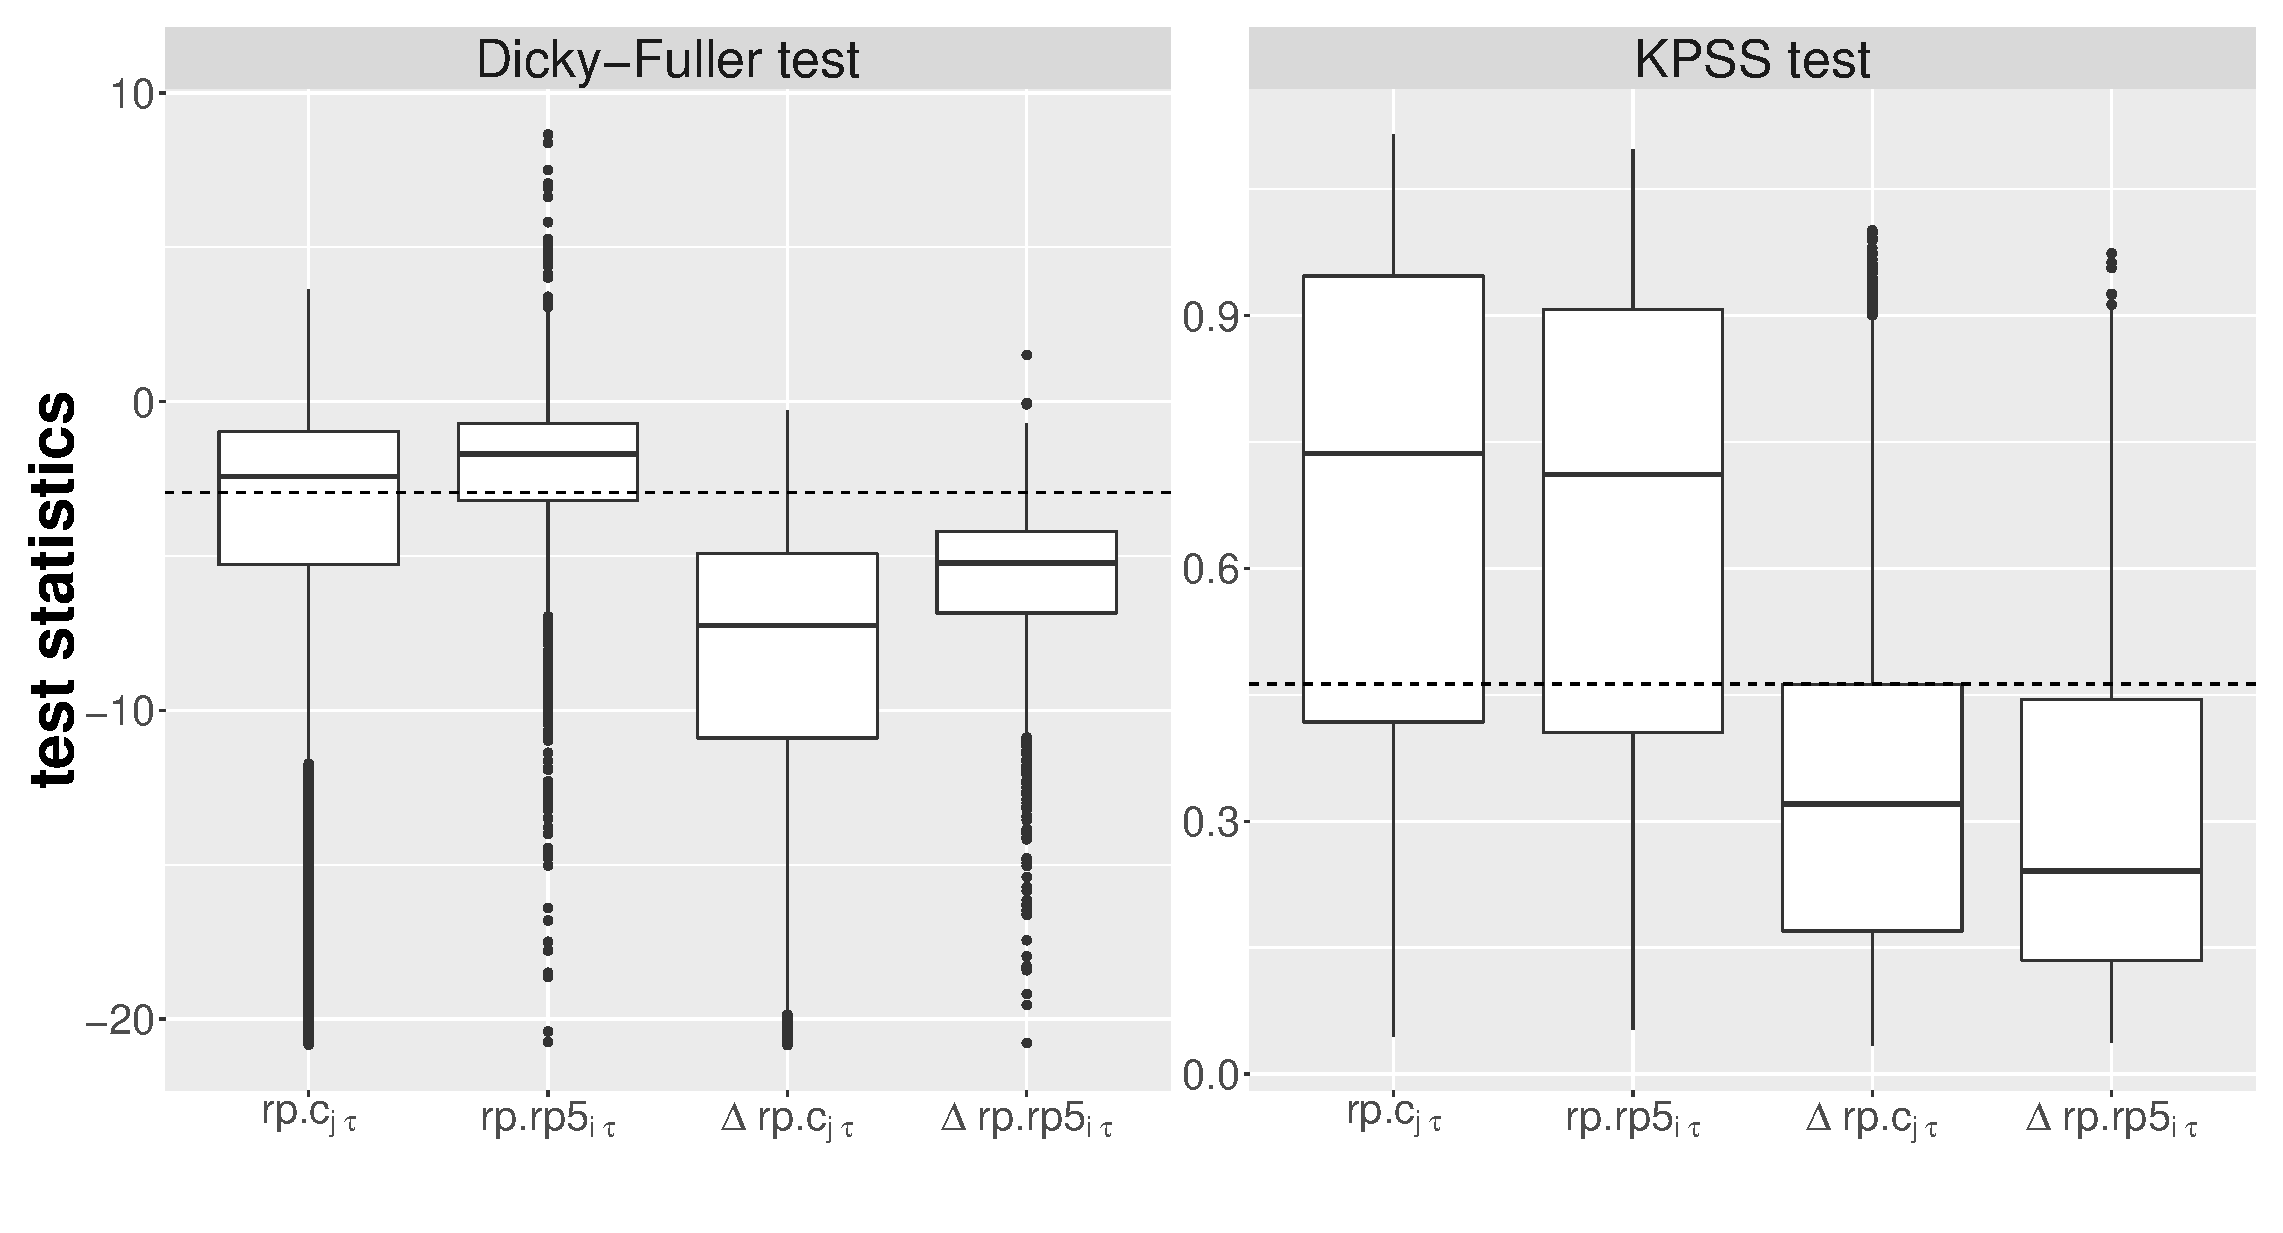
\includegraphics[width=\textwidth]{figures/stationarity_test/drift.eps}
    \caption{Statistical tests for the stationarity of rp series. Each test is applied on every individual rp series, and the test statistics are presented. Meanwhile, the $5 \%$ critical value for each test is shown as the dashed horizontal line. Both tests suggest that publication rp.c and scholar rp.rp5 are likely to be non-stationary. Meanwhile, both tests show evidence that the differenced series can be stationary. }
    \label{fig:stationarity_test}
\end{figure}

\begin{figure}[ht!]
    \centering
    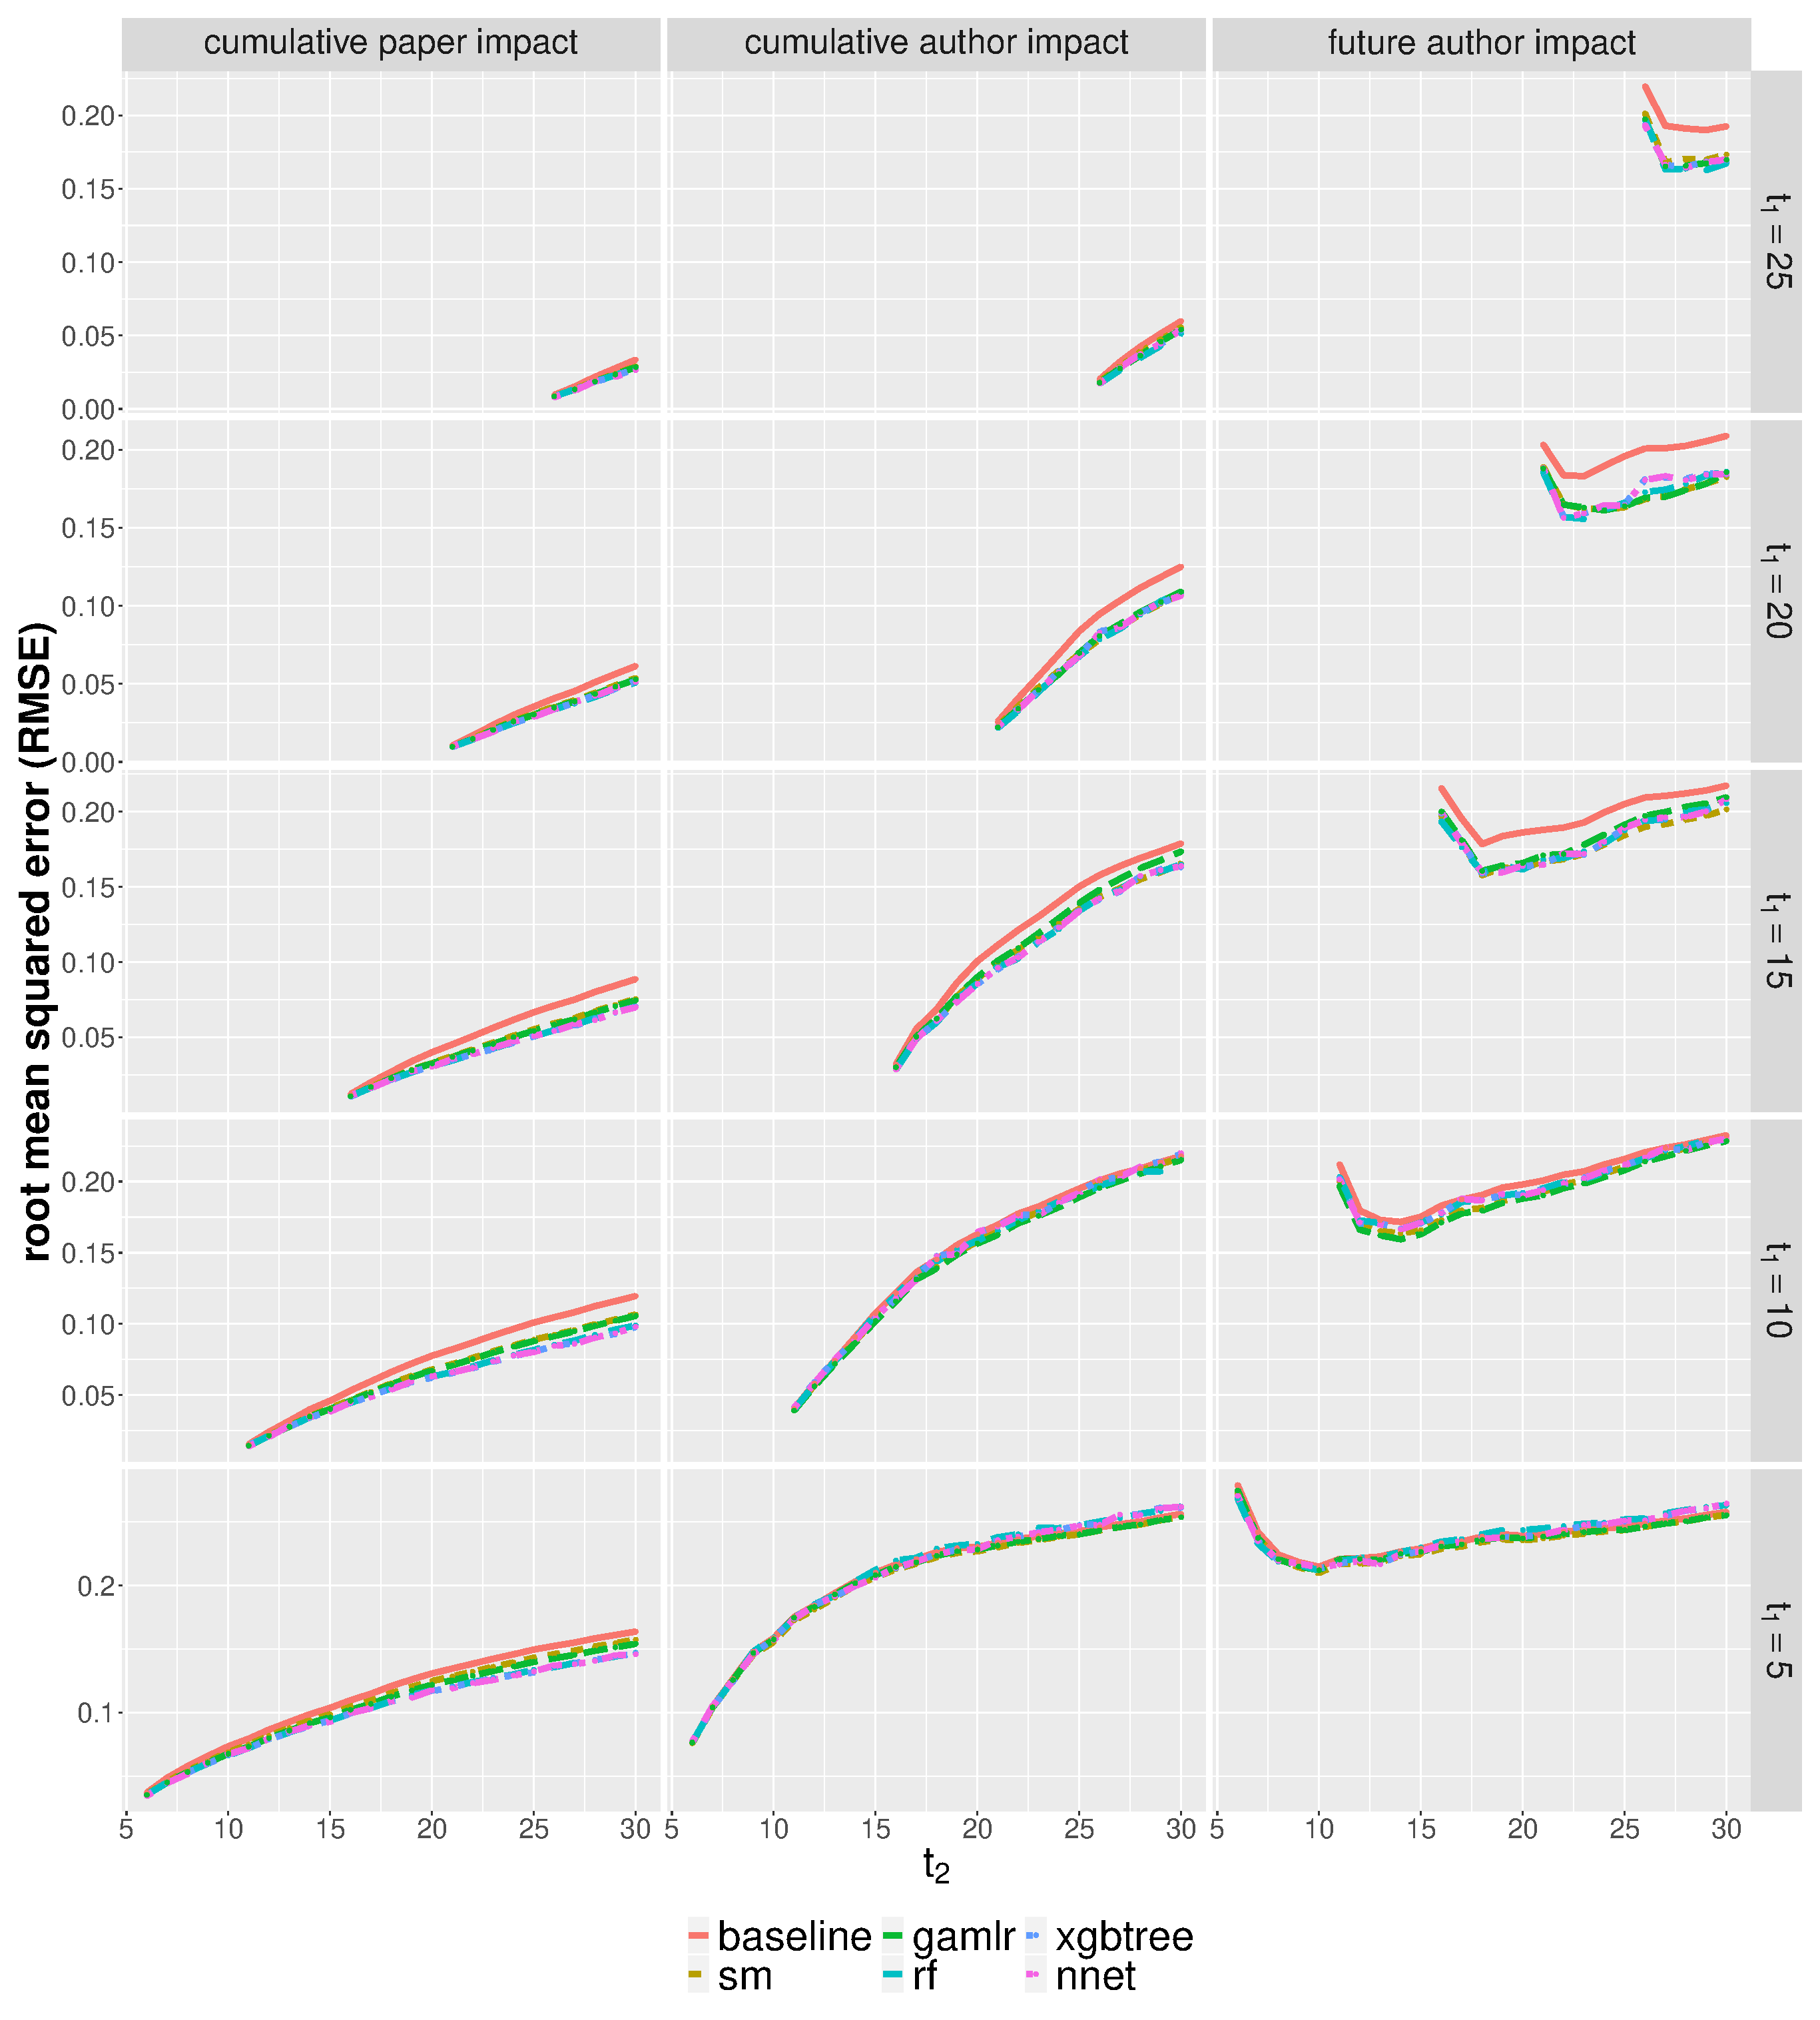
\includegraphics[width=\textwidth]{figures/pred_model/rmse_diff.eps}
    \caption{Root mean squared error (RMSE) of the predictive models. LASSO, ridge and elastic net are outperformed by Gamma LASSO, and hence are ignored for a better visualization.}
    \label{fig:pred_rmse}
\end{figure}

\begin{figure}[ht!]
    \centering
    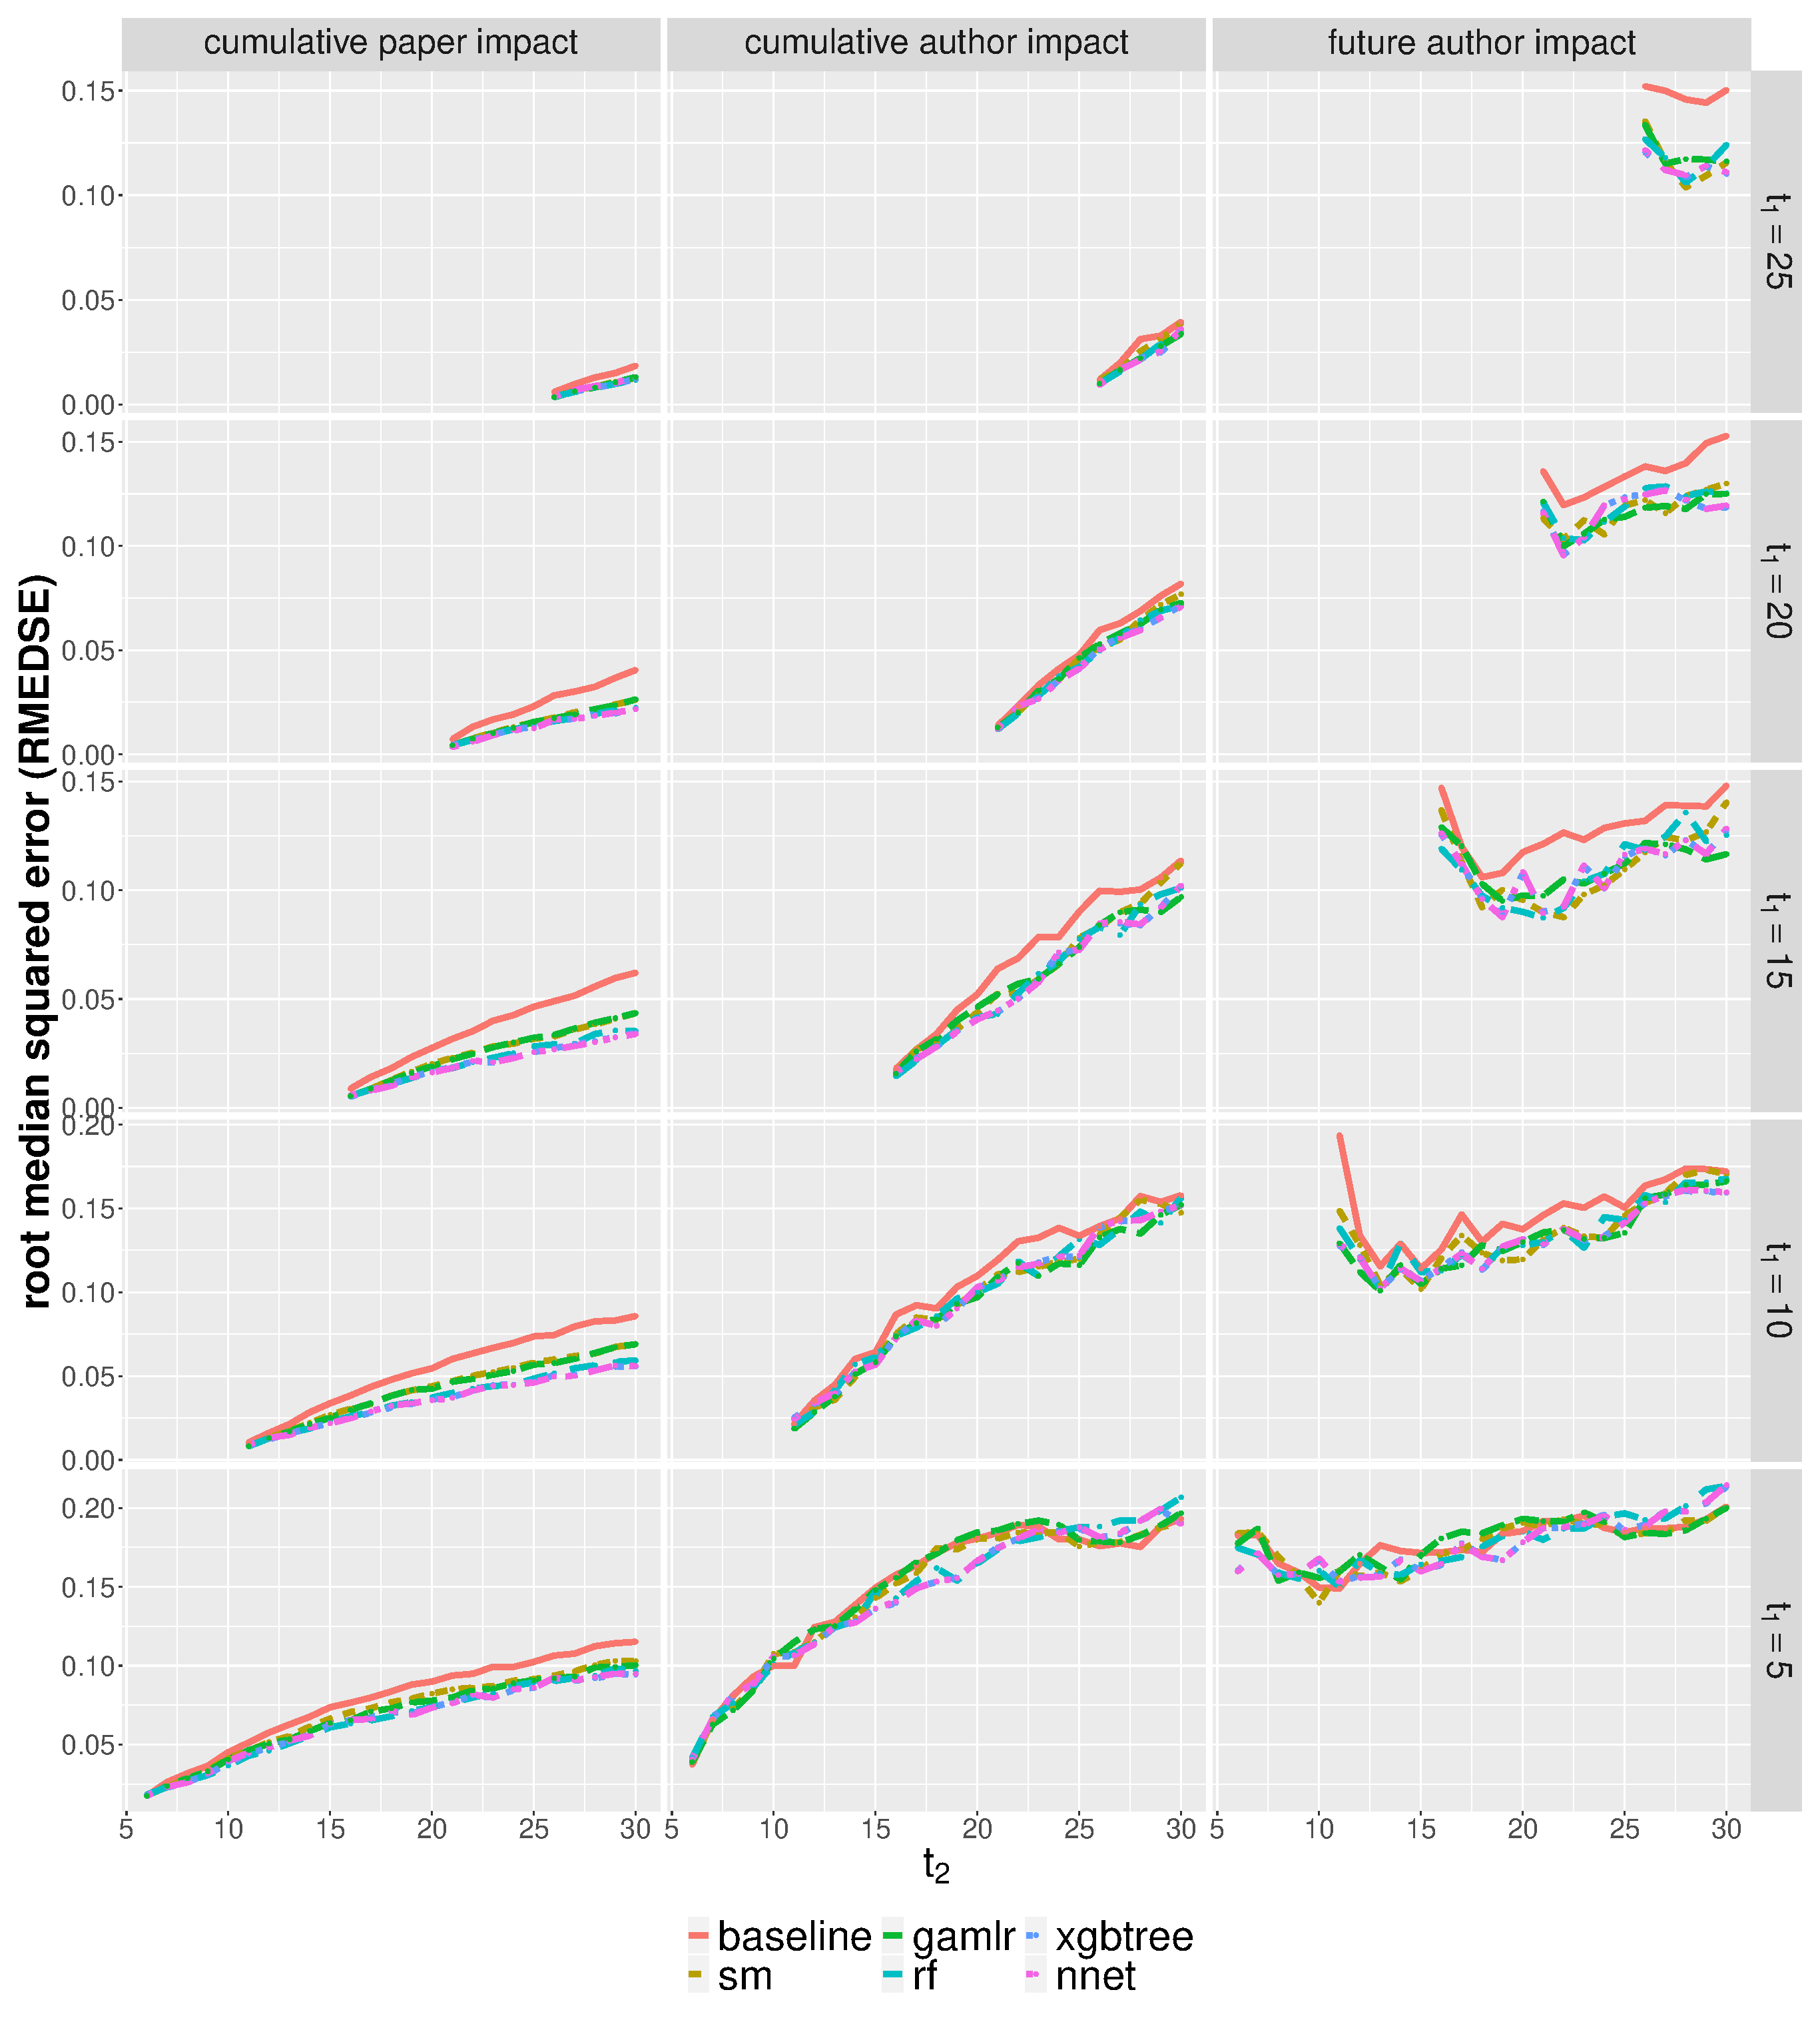
\includegraphics[width=\textwidth]{figures/pred_model/medse_diff.eps}
    \caption{Root median squared error (RMEDSE) of the predictive models. LASSO, ridge and elastic net are outperformed by Gamma LASSO, and hence are ignored for a better visualization.}
    \label{fig:pred_medse}
\end{figure}

\begin{figure}[ht!]
    \centering
    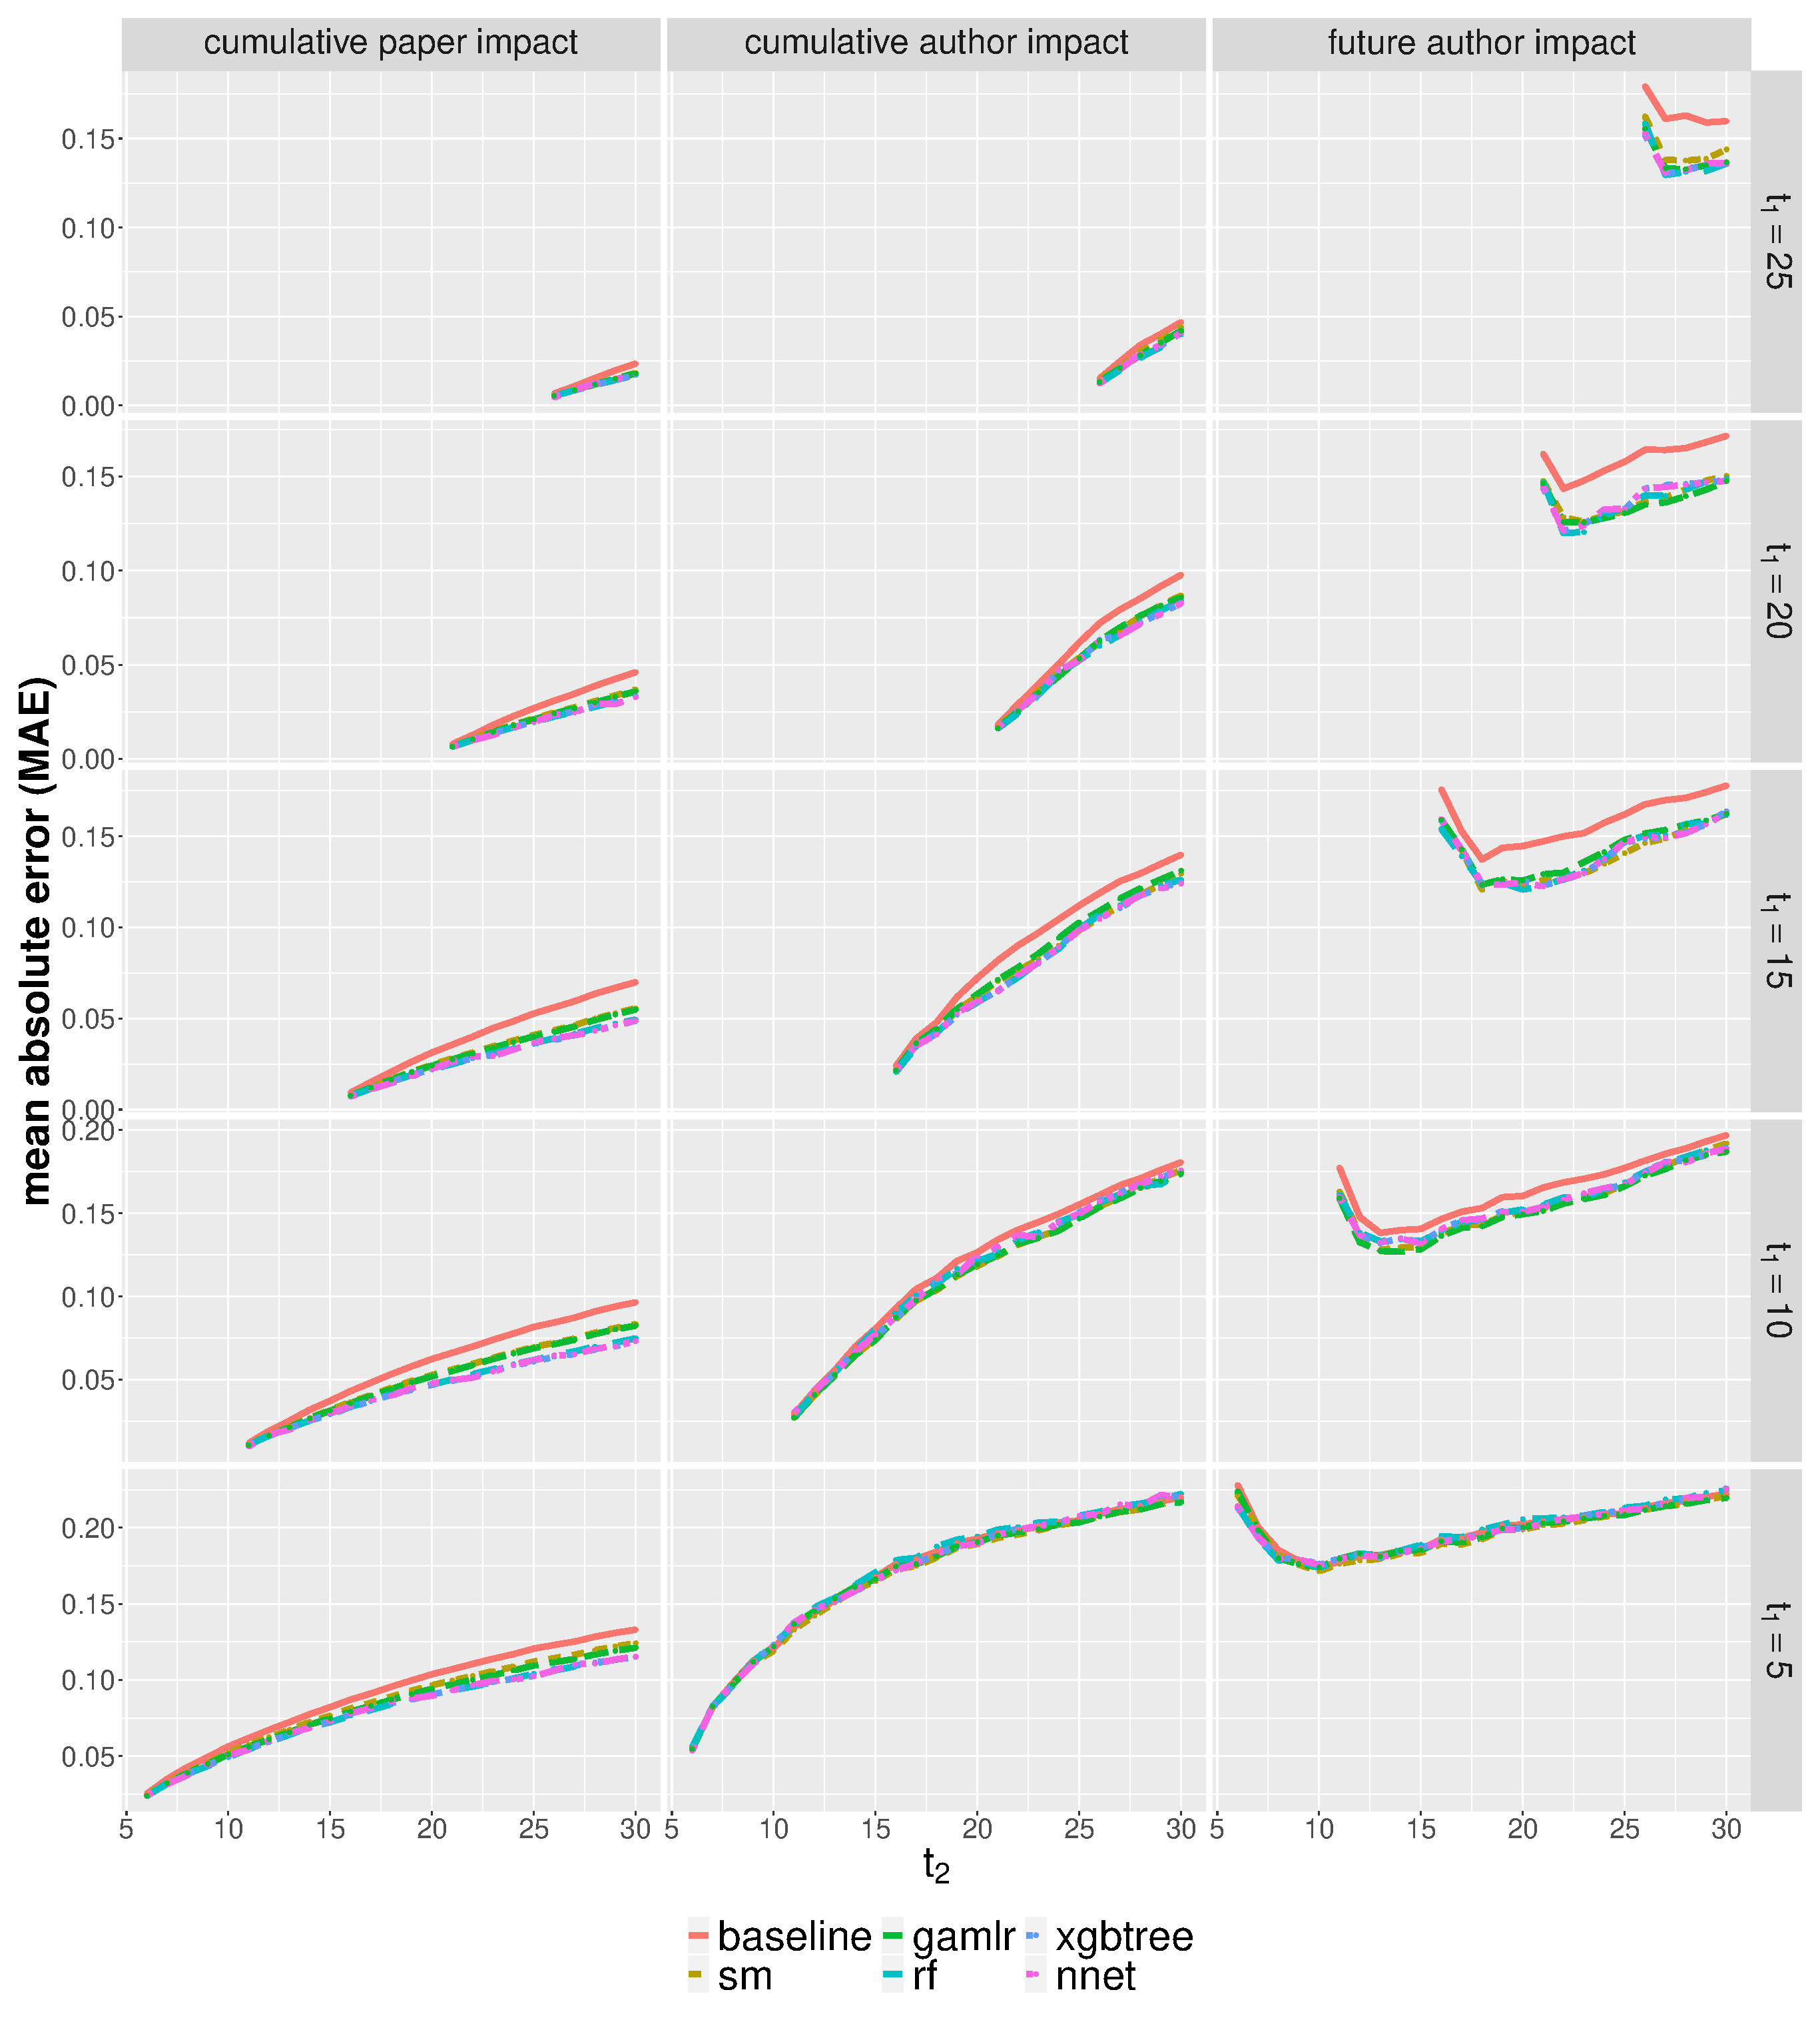
\includegraphics[width=\textwidth]{figures/pred_model/mae_diff.eps}
    \caption{Mean absolute error (MAE) of the predictive models. LASSO, ridge and elastic net are outperformed by Gamma LASSO, and hence are ignored for a better visualization.}
    \label{fig:pred_mae}
\end{figure}

\iffalse
\clearpage
Three effects may lead to the non-stationarity of rank percentile for scholars are:
\begin{itemize}
  \item Seniority effect of scholars: senior scholars can attract more citations than junior scholars. In figure \ref{fig:seniority}, we see that senior authors (e.g. those starting their careers in 1980s) do not have an advantage over junior authors (e.g. those starting their careers in 2000s). 
  \item Time effect: papers published more recently attract more citations than papers published $20$ years ago. This maybe due to the fact that the entire scientific community is growing, and we have much more scholars now than $20$ years ago, which makes the paper visible to a larger audience and potentially attracts more citations. Meanwhile, as Internet and especially social media becomes vital, papers now have much better visibility than those $20$ years ago. Figure \ref{fig:environment} shows that for the scholars starting their careers in $1980$, more recent papers attract more citations than old papers. Since we've already filtered out the seniority effect of the scholars, this is result from external effects. 
  \item Number of publications: scholars now tend to produce more publications than scholars say $20$ years ago. Evidence is shown in figure \ref{fig:npub}. 
\end{itemize}
We now fix the bias from the time effect and number of publications, in order to get stationary rank percentile indicators for scholars. Let's say we have a scholar $i$ who starts his/her career in physical year $Y_i$. For a paper $j$ that the scholar publishes in physical year $Y_j$, we calculate its rank percentile rp.c$_{j5}$ where the benchmark contains all the papers that are published in year $Y_j$. By restricting the benchmark in such way, we potentially remove the time effect. We repeat the process for all the papers of scholar $i$ that are published by age $t$ and obtain the metric $\sum_{j=1}^{N_t^{(i)}} \text{rp.c}_{j5}$. Furthermore, we calculate a rank percentile indicator rp.p$_{it}$ based on the number of publications by age $t$, and the benchmark is all the scholars who start their careers in physical year $Y_i$. Finally, we have the evaluation metric m$_{it} = \text{rp.p}_{it} \cdot \sum_{j=1}^{N_t^{(i)}} \text{rp.c}_{j5}$. The rank percentile indicator, denoted as rp.rp5, can be then computed based on m$_{it}$ and the benchmark is all or biology. 

Figure \ref{fig:compare_autrp} shows various types of scholar rank percentile indicators. Both rp.c and rp.h, that are based on total citations and h-index, show advantages for junior scholars due to the reasons explained above. However, rp.rp5 seems to be stationary. 


\begin{figure}[h!]
     \centering
     \begin{subfigure}[b]{0.48\textwidth}
         \centering
         
\includegraphics[width=\textwidth]{figures/exploratory/seniority_age5.eps}
         \caption{Total citations by age $5$ for papers published in $2012$}
     \end{subfigure}
     \hfill
     \begin{subfigure}[b]{0.5\textwidth}
         \centering
         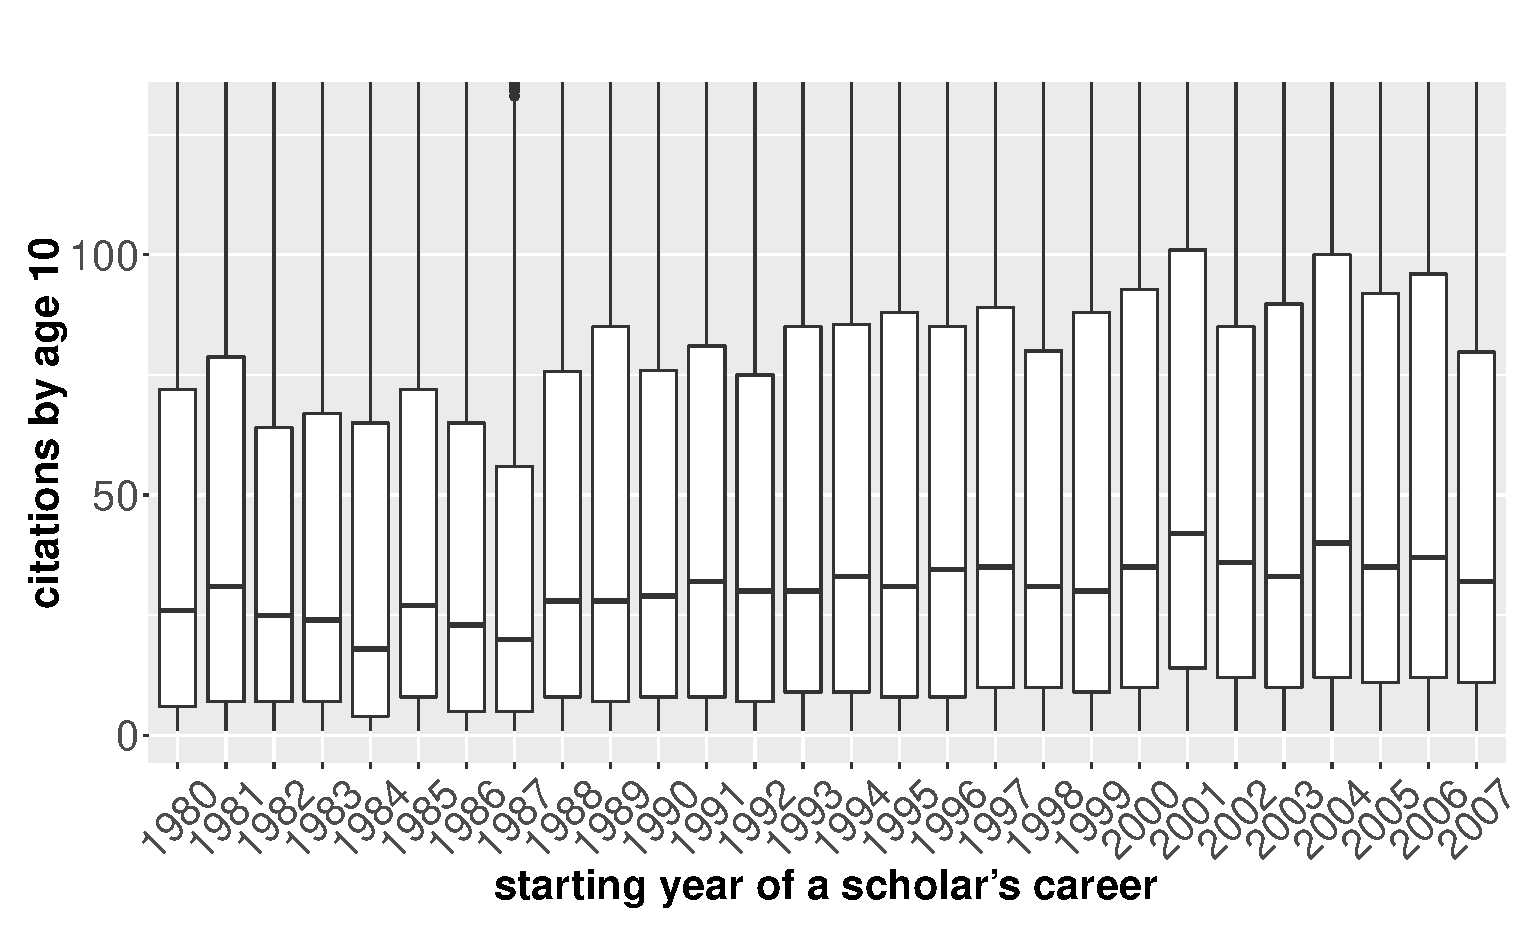
\includegraphics[width=\textwidth]{figures/exploratory/seniority_age10.eps}
         \caption{Total citations by age $10$ for papers published in $2007$}
     \end{subfigure}
    \caption{Seniority effect of scholars. The x-axis indicates starting years of careers of the corresponding authors. There's no evidence that senior scholars can attract more citations than junior scholars.}
    \label{fig:seniority}
\end{figure}

\begin{figure}[h!]
     \centering
     \begin{subfigure}[b]{0.48\textwidth}
         \centering
         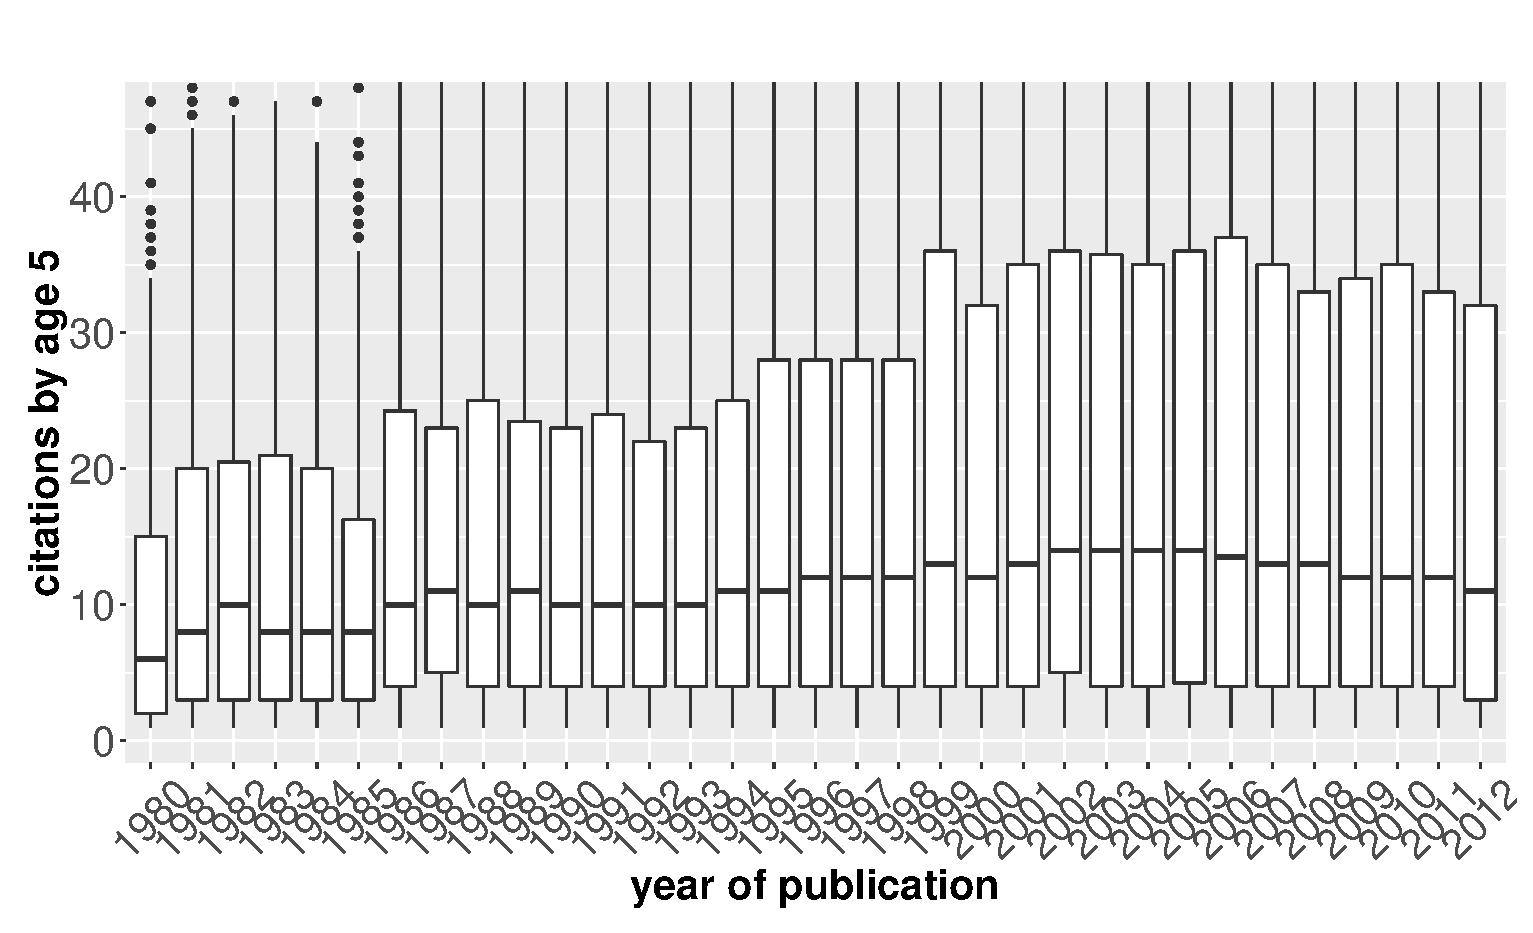
\includegraphics[width=\textwidth]{figures/exploratory/environment_age5.eps}
         \caption{Total citations by age $5$}
     \end{subfigure}
     \hfill
     \begin{subfigure}[b]{0.48\textwidth}
         \centering
         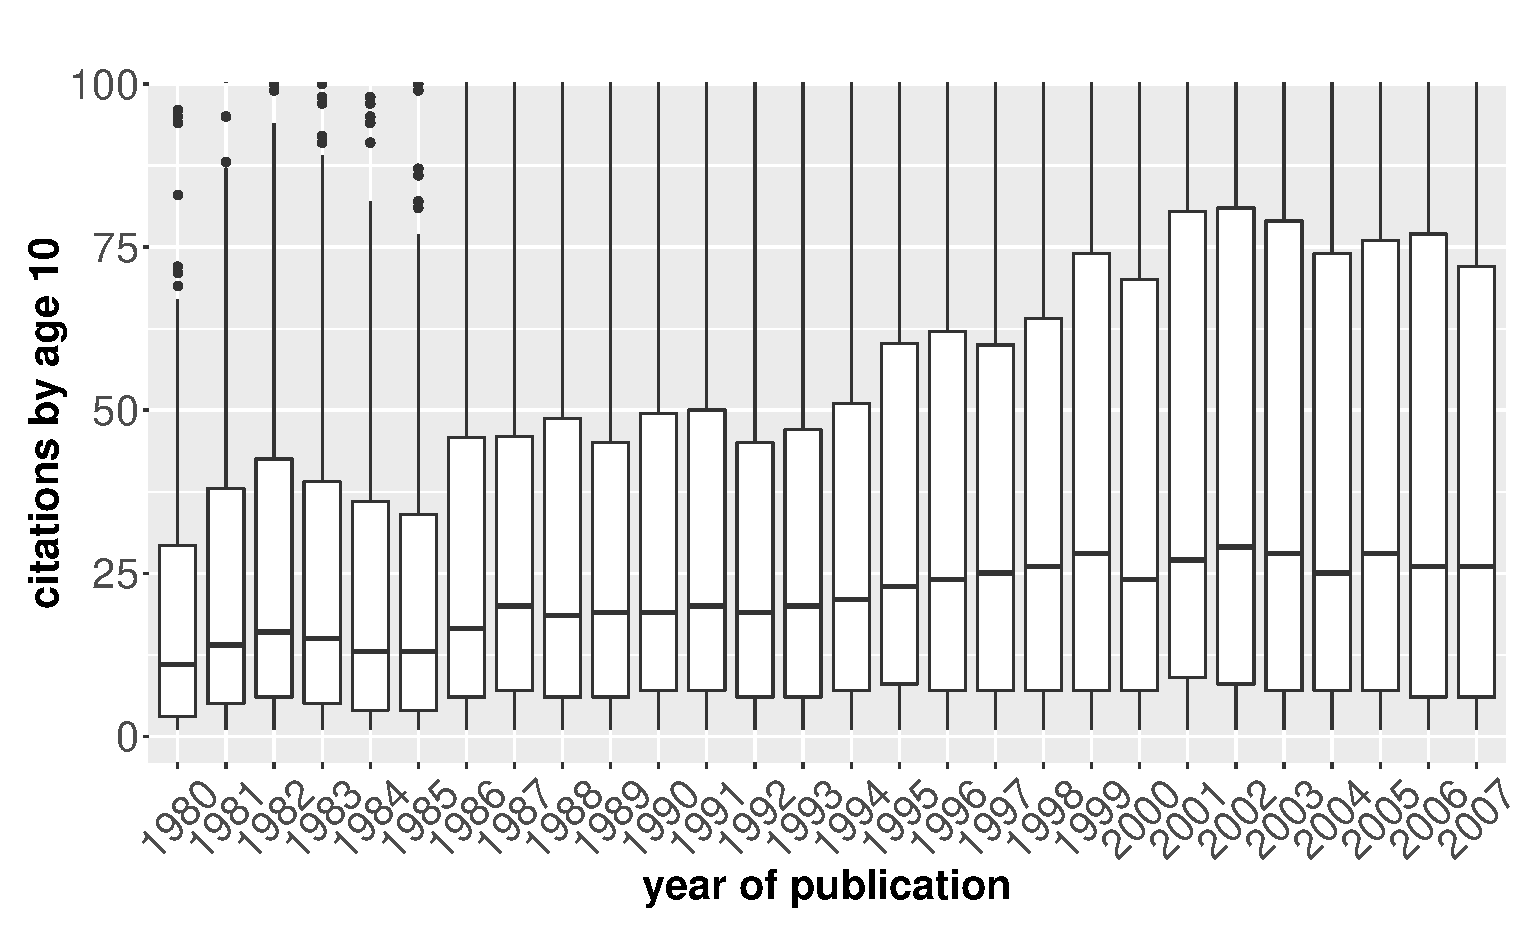
\includegraphics[width=\textwidth]{figures/exploratory/environment_age10.eps}
         \caption{Total citations by age $10$}
     \end{subfigure}
    \caption{Time effect. We consider the citations of the papers published by scholars who start their careers in year $1980$. The x-axis indicates the years of publication for their papers. We observe that more recent papers attract more citations than old papers.}
    \label{fig:environment}
\end{figure}

\begin{figure}[h!]
     \centering
     \begin{subfigure}[b]{0.48\textwidth}
         \centering
         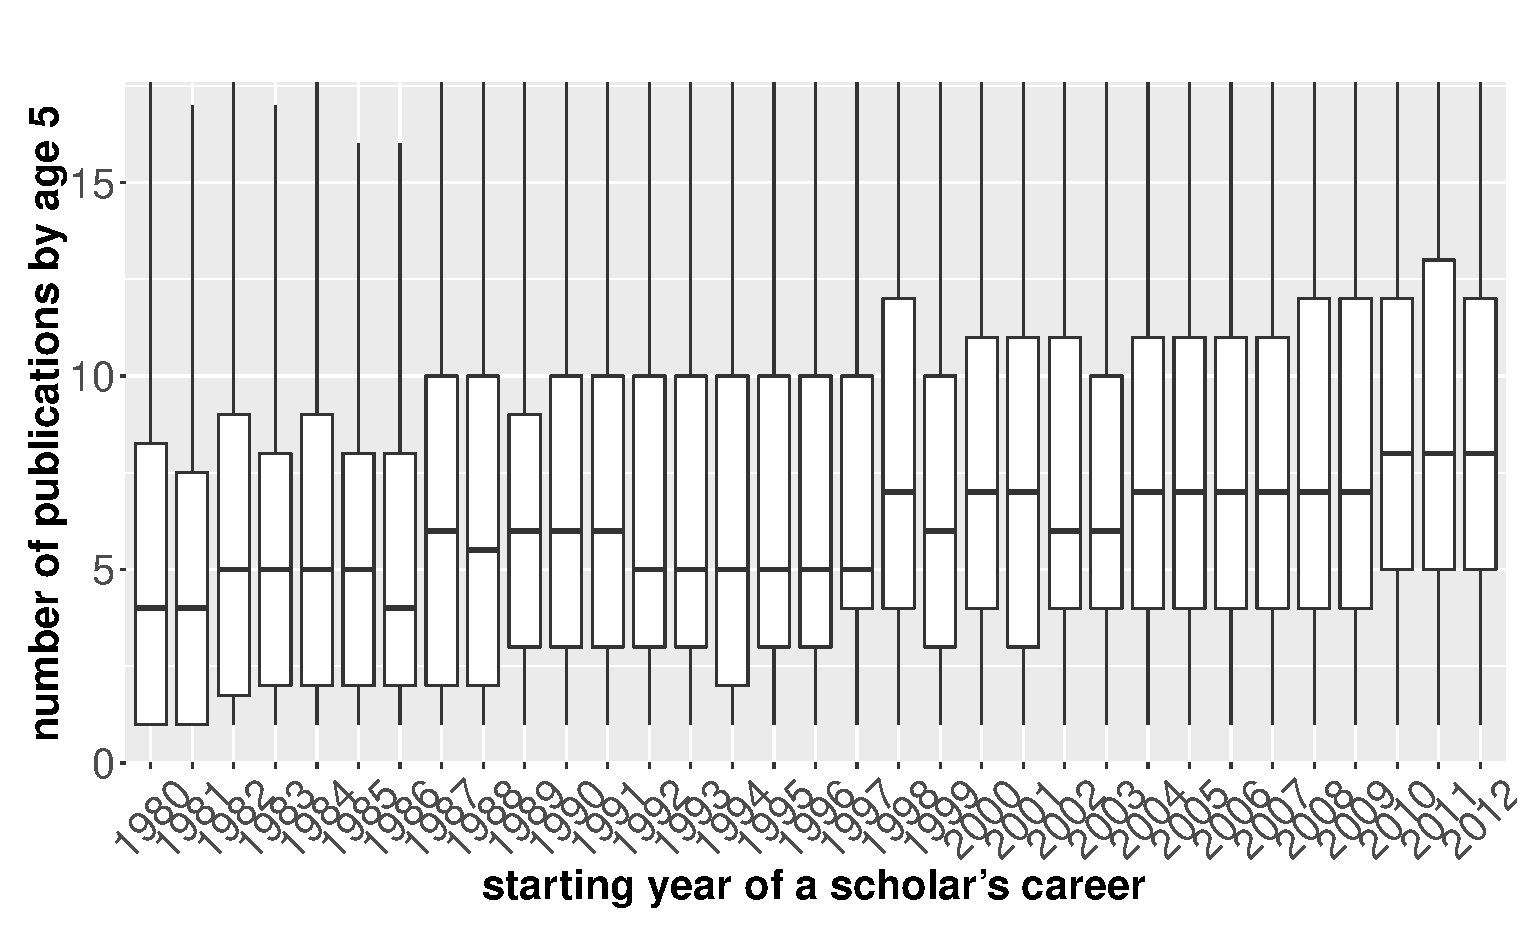
\includegraphics[width=\textwidth]{figures/exploratory/npub_age5.eps}
         \caption{Number of publications by age $5$}
     \end{subfigure}
     \hfill
     \begin{subfigure}[b]{0.48\textwidth}
         \centering
         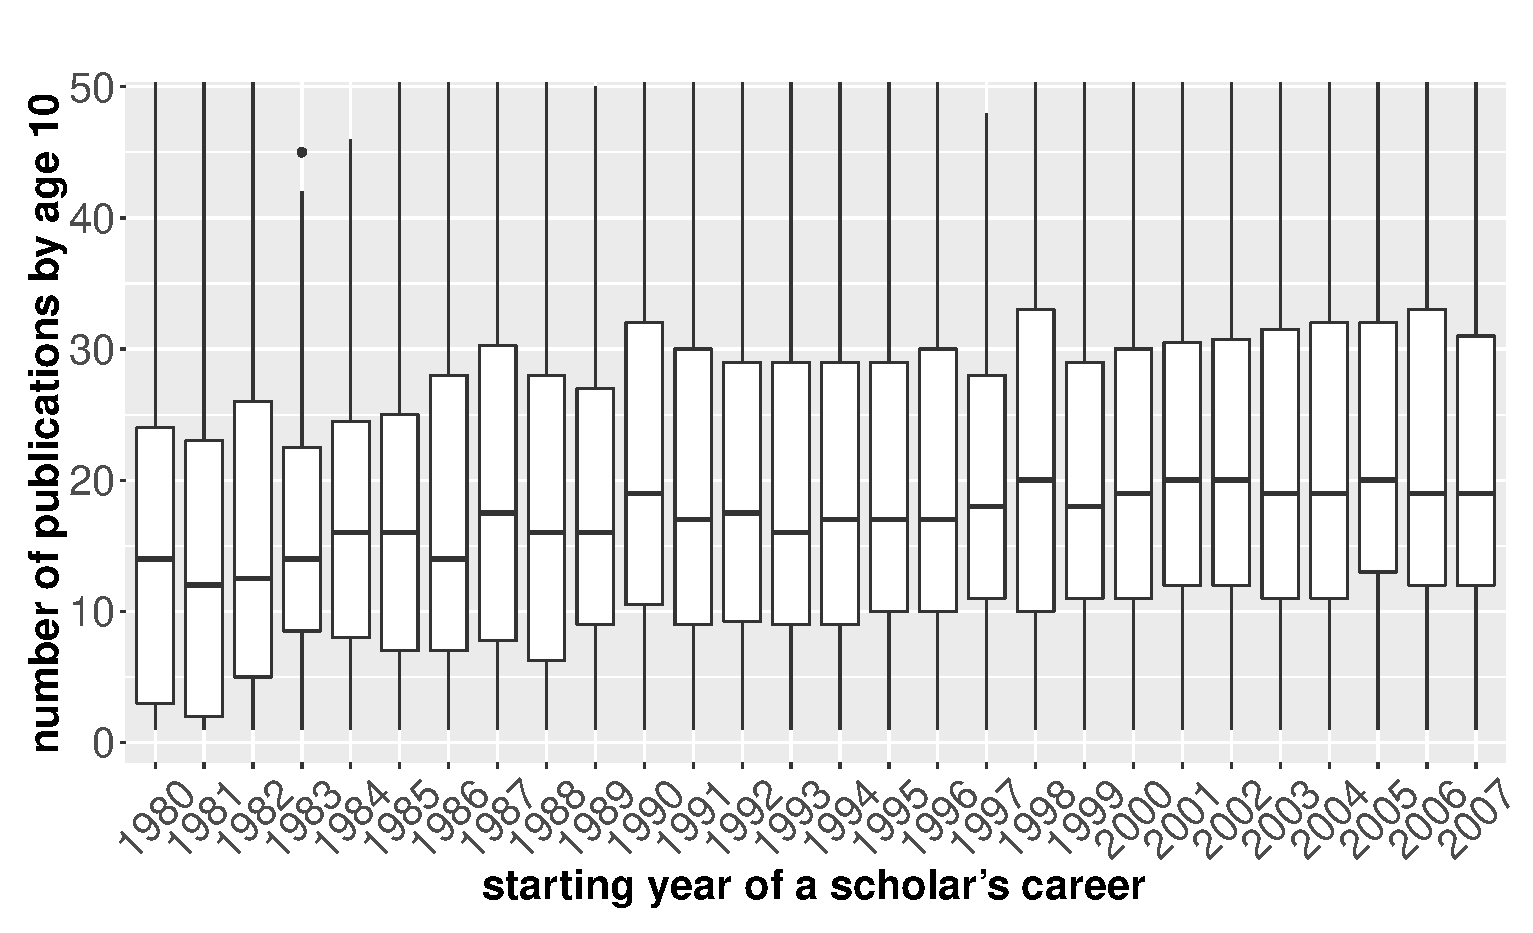
\includegraphics[width=\textwidth]{figures/exploratory/npub_age10.eps}
         \caption{Number of publications by age $10$}
     \end{subfigure}
    \caption{Number of publications. The x-axis indicates the starting years of careers of scholars. }
    \label{fig:npub}
\end{figure}


\begin{figure}[h!]
     \centering
     \begin{subfigure}[b]{0.48\textwidth}
         \centering
         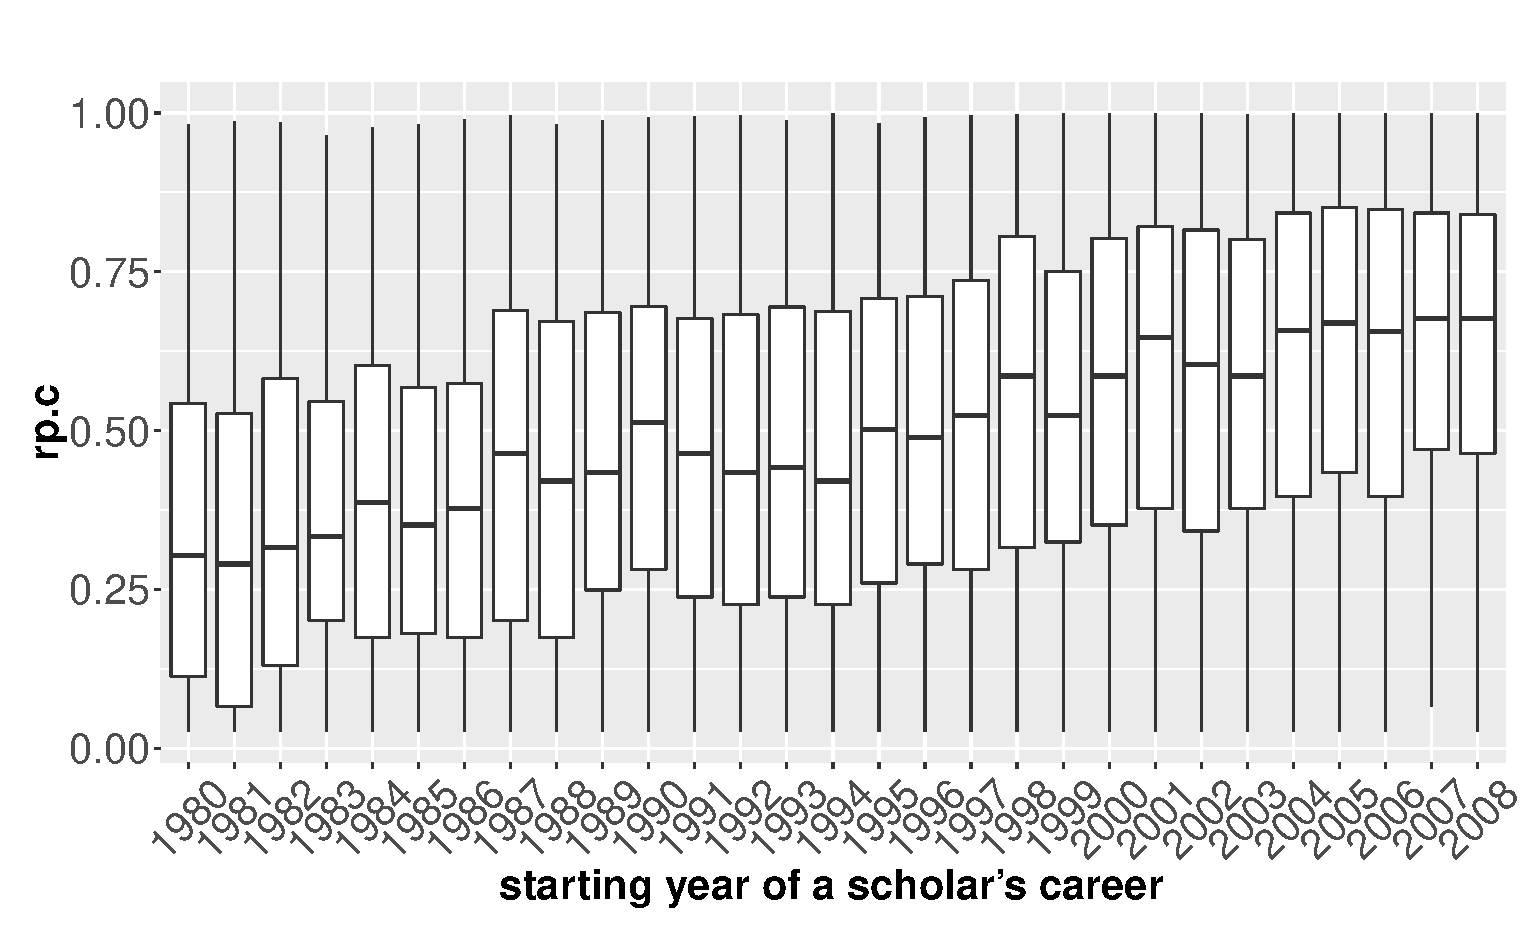
\includegraphics[width=\textwidth]{figures/exploratory/rpc_age5.eps}
         \caption{rp.c$_{i5}$}
     \end{subfigure}
     \hfill
     \begin{subfigure}[b]{0.48\textwidth}
         \centering
         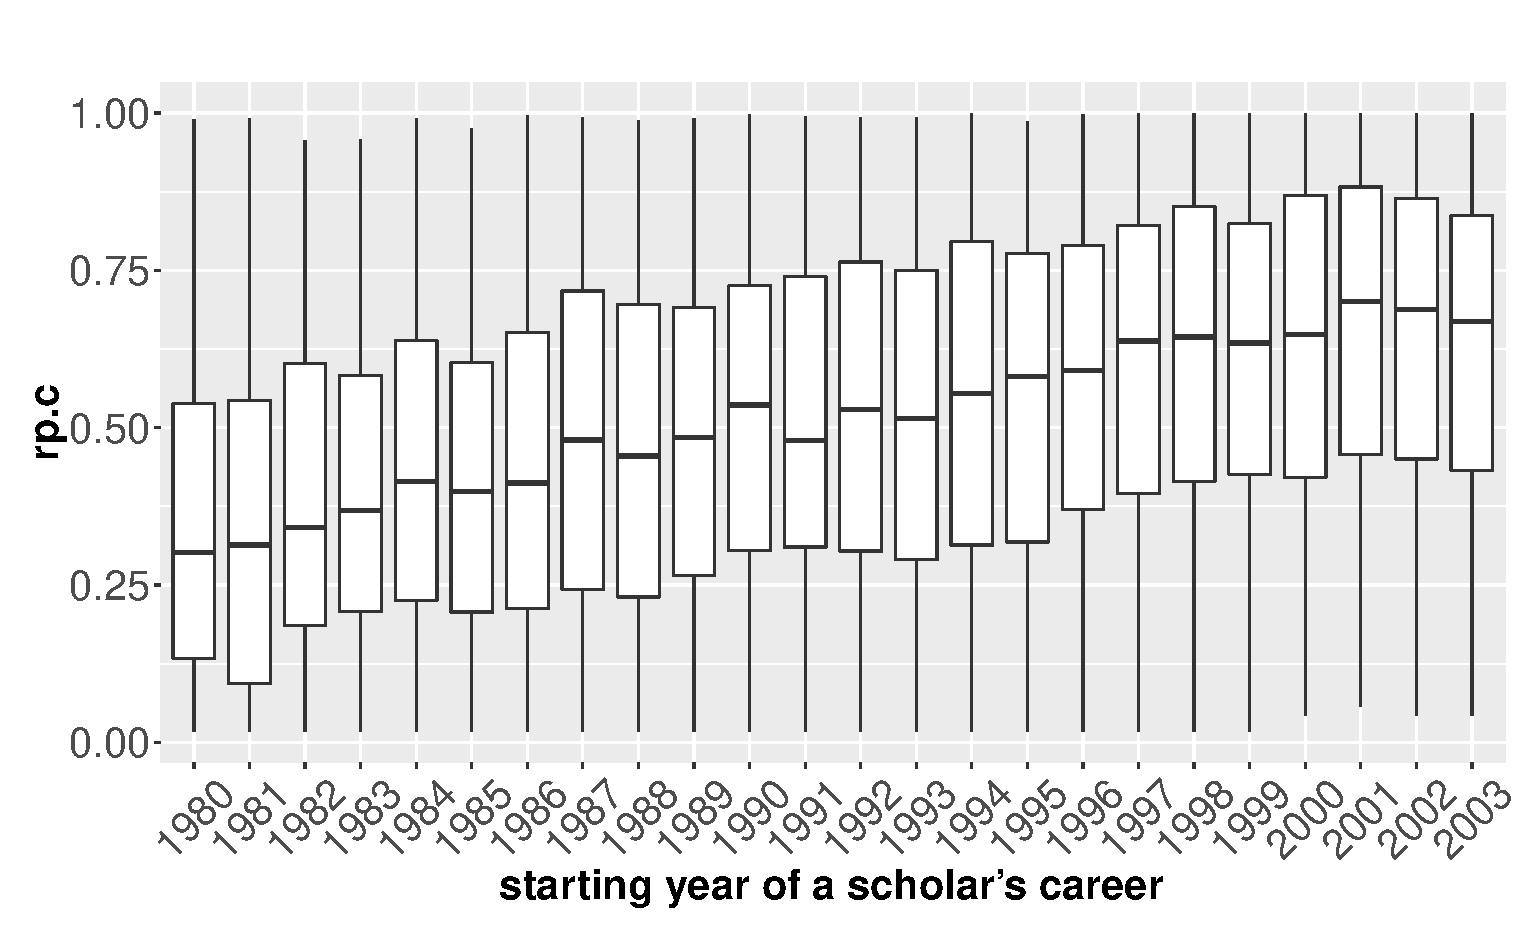
\includegraphics[width=\textwidth]{figures/exploratory/rpc_age10.eps}
         \caption{rp.c$_{i10}$}
     \end{subfigure}
     \hfill
      \begin{subfigure}[b]{0.48\textwidth}
         \centering
         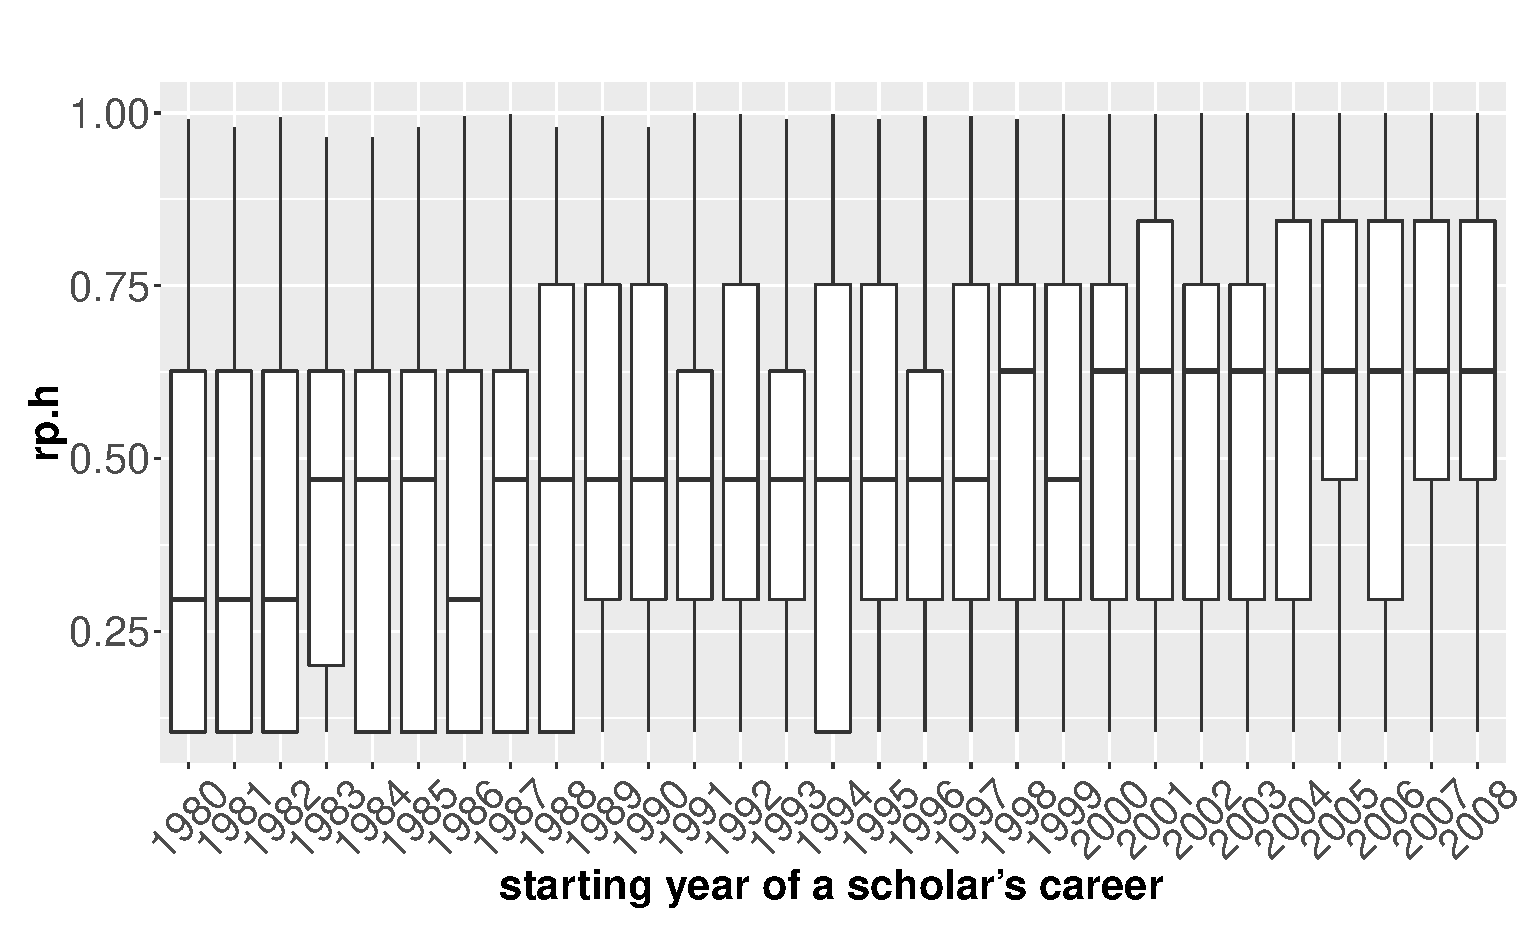
\includegraphics[width=\textwidth]{figures/exploratory/rph_age5.eps}
         \caption{rp.h$_{i5}$}
     \end{subfigure}
     \hfill
     \begin{subfigure}[b]{0.48\textwidth}
         \centering
         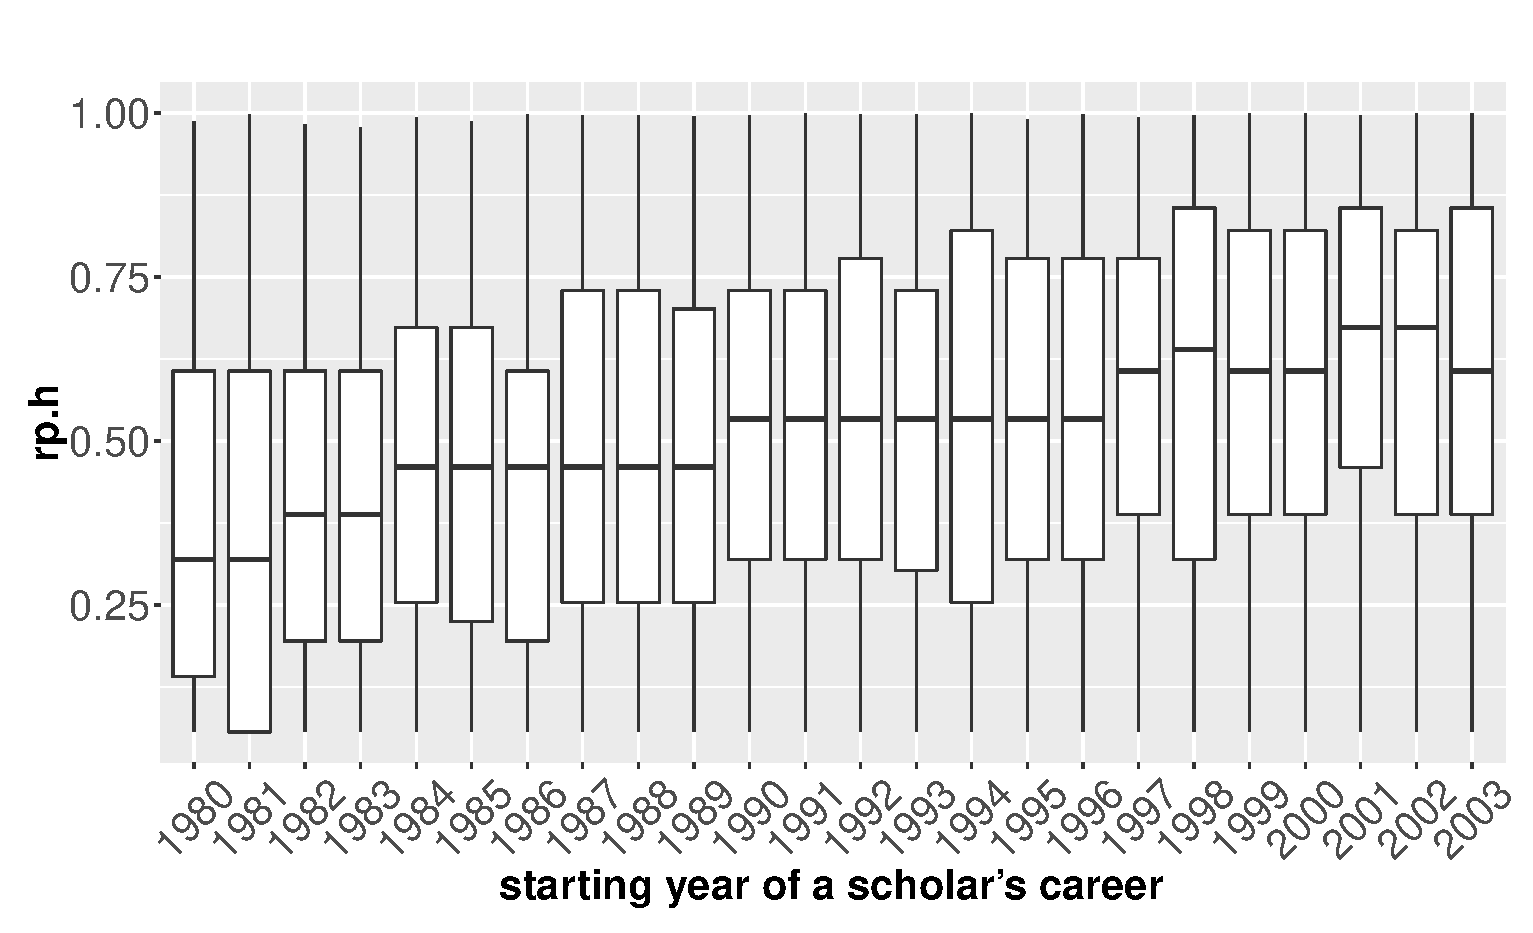
\includegraphics[width=\textwidth]{figures/exploratory/rph_age10.eps}
         \caption{rp.h$_{i10}$}
     \end{subfigure}
      \hfill
      \begin{subfigure}[b]{0.48\textwidth}
         \centering
         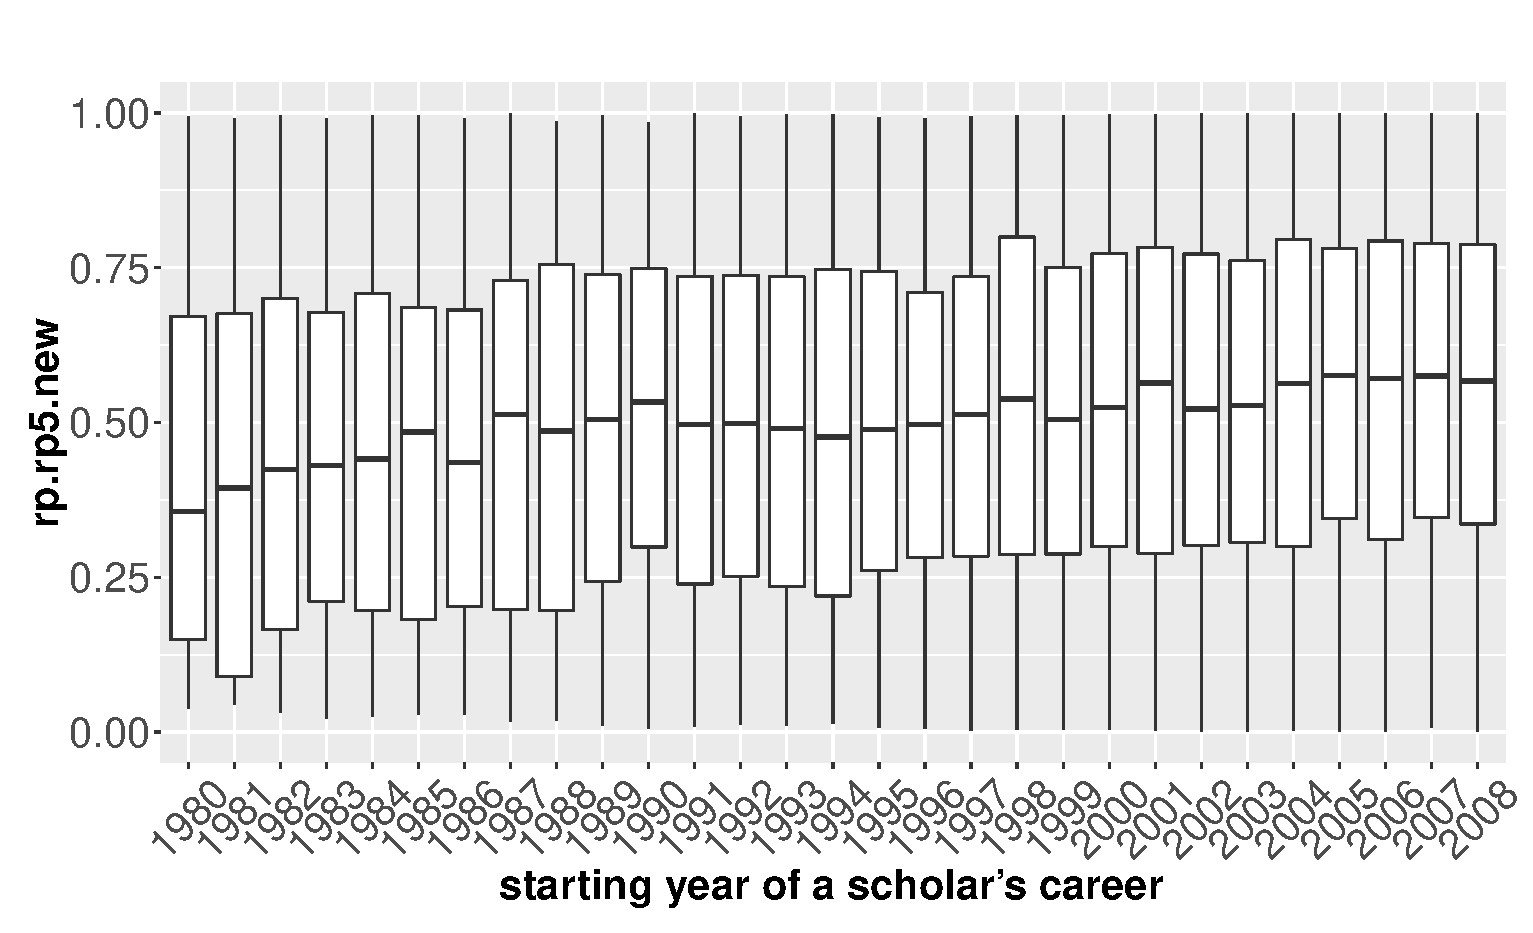
\includegraphics[width=\textwidth]{figures/exploratory/rprp5new_age5.eps}
         \caption{rp.rp5$_{i5}$}
     \end{subfigure}
     \hfill
     \begin{subfigure}[b]{0.48\textwidth}
         \centering
         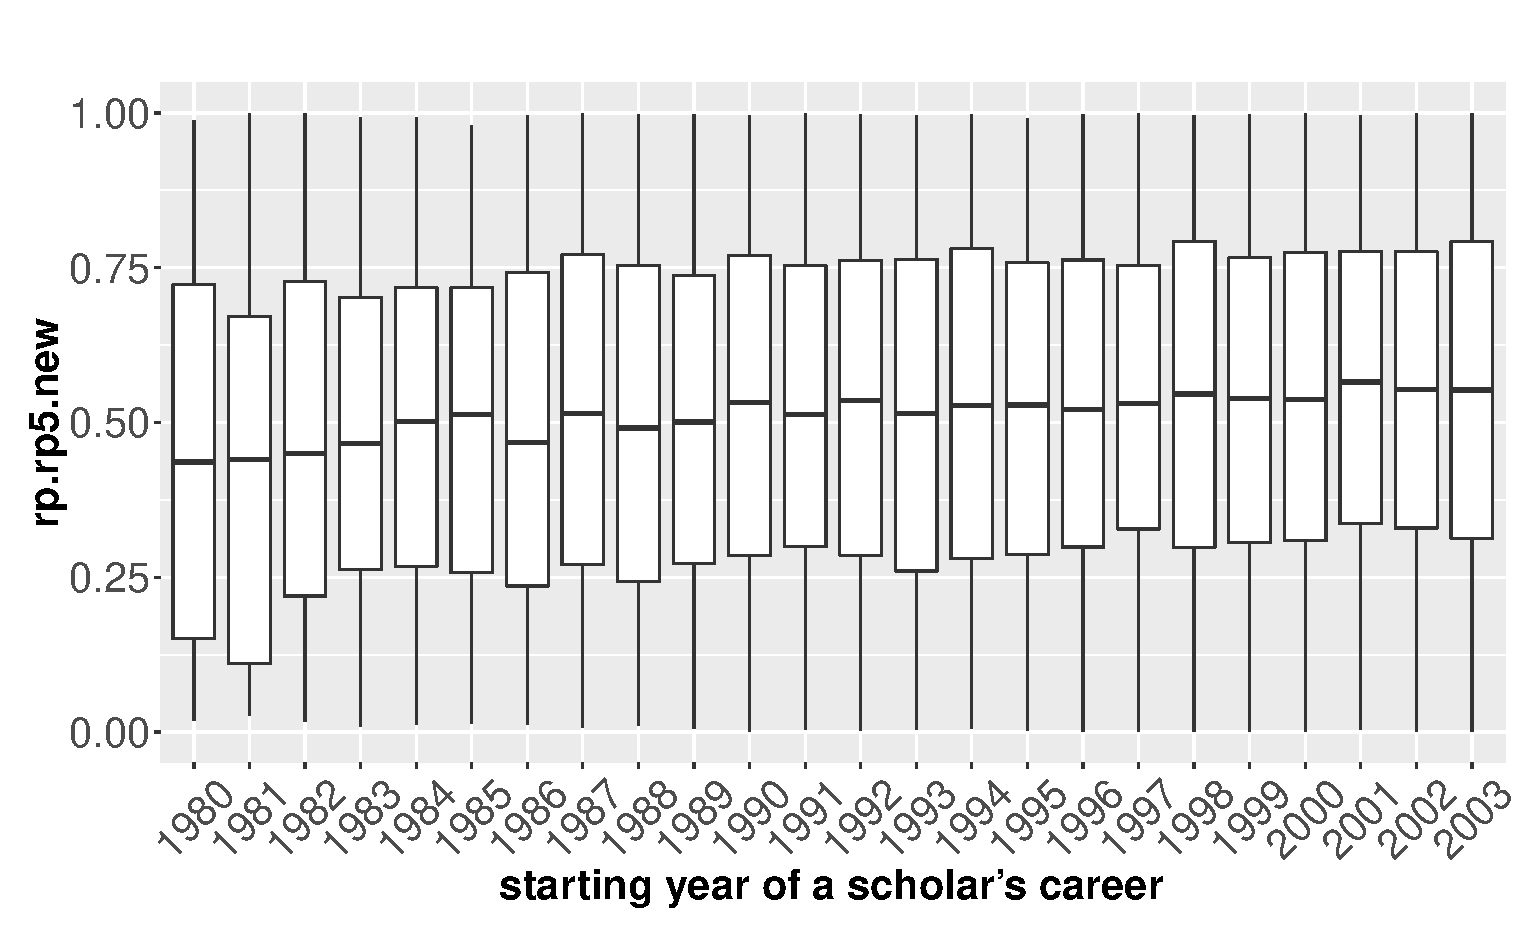
\includegraphics[width=\textwidth]{figures/exploratory/rprp5new_age10.eps}
         \caption{rp.rp5$_{i10}$}
     \end{subfigure}
    \caption{Different types of rank percentile indicators for scholars. rp.rp5 is stationary, while the other two are not.}
    \label{fig:compare_autrp}
\end{figure}

\fi
\end{refsection}